\section{Empirical Benchmarks and Real-World Validation}
\label{sec:results}

Empirical validation must bridge mathematical theory to biological reality.
Benchmarking recombination algorithms requires evaluating multiple distinct biological dimensions across the complete reticulation event.
Binary alerts conceal structural errors.
An algorithm can easily trigger alarms on mutational rate variation, invert parental polarity, or fragment a single conversion tract into multiple spurious breakpoints while claiming high empirical sensitivity.
Objective standards prevent metric gaming.
We formalize performance across four foundational dimensions: alignment-level detection on clonal nulls, breakpoint cardinality, informational spatial accuracy, and directed sequence identity (Table~\ref{tab:evaluation_framework}).

\begin{table*}[t!]
\caption{Formal benchmark scoring framework across reticulation dimensions. Performance is evaluated across four primary biological dimensions to prevent methodological gaming: alignment-level classification under non-recombinant nulls, breakpoint cardinality, spatial boundary accuracy under sequence information bounds, directed triad attribution, ghost donor introgression, and ancestral event consolidation.}
\label{tab:evaluation_framework}
\centering
\small
\begin{tabularx}{\textwidth}{>{\raggedright\arraybackslash}p{2.5cm} >{\raggedright\arraybackslash}p{3.2cm} Y Y}
\toprule
\textit{Dimension} & \textit{Biological Question} & \textit{Formal Benchmark Criterion} & \textit{Mathematical Scoring Metric} \\
\midrule
Alignment-Level Detection & Does the alignment contain authentic horizontal genetic exchange? & Complete rejection of non-recombinant clonal nulls under heterotachy, APOBEC bursts, Darwinian selection, and molecular clock evolution. High sensitivity on true mosaics. & Binary classification with false positive rate $\text{FPR} = \text{FP} / N_{\text{null}} = 0.00\%$ at $\alpha = 0.05$ and sensitivity $\text{TPR} = \text{TP} / N_{\text{rec}}$. \\
\addlinespace
Breakpoint Cardinality & How many recombination breakpoints occurred along the chromosome? & Strict agreement between predicted and true changepoint counts. Over-splitting and spurious fragmentation are penalized as false alarms. & Bijective bipartite matching via Hungarian algorithm on cost $C_{ij} = 1 - s(E_i, \hat{E}_j)$ with cardinality penalty $\Delta K = |\hat{K} - K_{\text{true}}|$. \\
\addlinespace
Breakpoint Localization & Where are the boundaries of horizontal genetic exchange located? & Informative SNP Jaccard Index ($J_{\text{SNP}}$) over flanking informative polymorphisms $[u_{\text{inf, left}}, u_{\text{inf, right}}]$. Contradictory SNP distance outside the plateau. & $J_{\text{SNP}} = \frac{|\mathcal{S}_{\text{true}} \cap \mathcal{S}_{\text{inferred}}|}{|\mathcal{S}_{\text{true}} \cup \mathcal{S}_{\text{inferred}}|}$; exact plateau containment ($E_{\text{SNP}} = 0 \iff J_{\text{SNP}} = 1.00$). \\
\addlinespace
Sequence Identity and Direction & Which sequence is the recombinant, which is the major parent, and which is the donor? & Directed triad attribution $(C, H, D)$ distinguishing recombinant child $C$, home recipient $H$, and donor parent $D$. Rejection of reciprocal 2-cycle cheats ($C \leftrightarrow D$). & Triad fidelity $S_{\text{triad}}$ with phylogenetic partial credit $w(X, Y)$ and physical transition contrast $\Delta d_{\text{home}} > 0, \Delta d_{\text{donor}} > 0$. \\
\addlinespace
Ghost Donor Introgression & Does the transferred sequence originate from an unsampled or extinct lineage? & Correct identification of unsampled donor ($D = \varnothing$) without framing innocent background outgroup sequences as false recombinant children. & Ghost recall $\mathbb{I}(\hat{D} = \text{Ghost})$ with background false alarm rate $\text{FPR}_{\text{bg}} = \text{FP}_{\text{bg}} / N_{\text{bg}} = 0.00\%$. \\
\addlinespace
Ancestral Event Consolidation & How many independent historical recombination events occurred in the cohort? & Grouping epidemiologically related descendant isolates sharing homologous parental lineages and overlapping breakpoints into a single ancestral event. & Interval overlap $\ge 50\%$ with compatible parental pair $(H, D)$ and consolidated event ratio $K_{\text{events}} / N_{\text{isolates}}$. \\
\bottomrule
\end{tabularx}
\end{table*}

Spatial precision demands metrics grounded in sequence information content instead of arbitrary distance thresholds.
Information bounds resolution.
Between adjacent informative polymorphisms that distinguish parental lineages, alignments contain zero phylogenetic signal, causing the log-likelihood profile to form an exact mathematical plateau.
Judging breakpoint accuracy through fixed nucleotide windows creates a false standard.
A rigid threshold penalizes exact calls in conserved regions while forgiving predictions that cross dozens of contradictory mutations in divergent genomes.
Instead, we evaluate spatial accuracy through the Informative SNP Jaccard Index ($J_{\text{SNP}}$), measuring the fraction of true informative polymorphisms recovered within the inferred boundary.
Whenever a predicted coordinate lands anywhere within the flanking informative plateau of the true exchange, the traversed SNP error is zero ($E_{\text{SNP}} = 0$), yielding $J_{\text{SNP}} = 1.00$.

Lineage attribution requires equal discipline.
Calling recombination on the wrong sequence or inverting the reticulation arrow represents total biological failure.
We evaluate directed triad fidelity ($S_{\text{triad}}$), requiring accurate identification of the recombinant child, the home recipient, and the donor parent.
Phylogenetic partial credit accounts for genealogical proximity, awarding proportional affinity when an algorithm identifies a close sister isolate within the same monophyletic clade.
Transposed child-donor cycles collapse to zero because deep inter-clade divergence extinguishes affinity.
To penalize over-splitting, predicted events are paired to ground truth through bijective bipartite matching via the Hungarian algorithm.
Unmatched predictions deflate precision ($\text{PPV}_{\mathcal{R}}$), while undetected exchanges depress recall ($\text{TPR}_{\mathcal{R}}$).
The individual dimensions unite into the composite Reticulation Fidelity Index ($\mathcal{R}_{F_1}$), providing an un-gameable benchmark standard (Materials and Methods, Section~\ref{subsec:methods_scoring_framework}).

\subsection{Coalescent Benchmarks: The Hyper-Recombination Paradox and Spatial Observability}
\label{subsec:posada_crandall_benchmark}

When recombination rates escalate toward the hyper-recombinant limit ($\rho \to \infty$), conventional intuition assumes that mosaic events should become trivial to detect.
The opposite is true.
Too much recombination looks like no recombination.
When an ancestral recombination graph shatters a chromosome into micro-tracts shorter than the distance between informative mutations, the spatial autocorrelation of phylogenetic affinity vanishes.
Lineages exchange identical alleles.
The sequence of pairwise differences collapses into an uncorrelated Poisson point process with constant rate $\bar{d}$.
Physically and mathematically, hyper-recombinant evolution becomes indistinguishable from clonal evolution under a molecular clock with site-to-site homoplasy.
Every changepoint detector searching for spatial clustering of affinity finds white noise.
The signal is not missed by imperfect heuristics.
The signal does not exist in the alignment.

Under Kingman's coalescent with recombination, ancestral partitions scale harmonically as $\mathbb{E}[N_{\text{part}}] \approx 1 + \rho \sum_{k=1}^{n-1} k^{-1}$.
For $n=10$ taxa at $\rho=64$, this shatters a 1,000-nucleotide alignment into $\sim 160$ independent genealogical segments.
Mean tract length compresses to $\bar{L}_{\text{tract}} \approx 6.25\text{ nt}$ (barely two codons).
In contrast, at population mutation rate $\theta = 10$ (pairwise divergence $p \approx 1\%$), informative polymorphisms occur roughly once every $\bar{\Delta}_{\text{SNP}} \approx 100\text{ nt}$.
Tract length is sixteen times smaller than mutational spacing ($\bar{L}_{\text{tract}} / \bar{\Delta}_{\text{SNP}} \approx 0.06$).
Over 94\% of simulated coalescent segments contain zero segregating sites.
The tract length sits far below the spatial Nyquist sampling rate of the mutational process.
As $\rho \to \infty$, the genealogical correlation length $L_{\text{corr}} \sim 1/\rho \to 0$, destroying sequence memory.
Penalizing algorithms for omitting silent micro-tracts mistakes unmutated genealogical history for observable data.

This physical boundary requires classifying analysis difficulty across three independent planes rather than tracking crude binary alerts.
In Plane 1 (Detection Identifiability), statistical power depends on informative polymorphism density ($\delta_{\text{inf}} = S_{\text{inf}} / L$) and four-gamete incompatibility prevalence ($\Upsilon_{4G}$).
Alignments with $S_{\text{inf}} < 3$ are informationally sterile.
The data cannot reject tree space.
In Plane 2 (Breakpoint Localization), spatial accuracy is bounded by the physical Shannon limit ($\Delta \tau_{\text{lim}} = s_{\text{right}} - s_{\text{left}}$), representing the interval between parental distinguishing polymorphisms flanking the exchange.
Predictions inside $[\tau - \Delta_{\text{left}}, \tau + \Delta_{\text{right}}]$ achieve optimal zero-error containment ($J_{\text{SNP}} = 1.00$).
Tracts lacking distinguishing mutations ($N_{\text{inf}}(\mathcal{I}) = 0$) represent unobservable ghost exchanges.
In Plane 3 (Lineage Attribution), parental contrast depends on patristic divergence ($d_{H, D} = d_{\text{tree}}(H, D)$) and donor clade uniqueness margin ($\mu_{\text{donor}}$).
Midpoint crossovers ($\eta_{\text{pol}} \approx 1.0$) introduce mathematical role symmetry, whereas asymmetric cassettes ($\eta_{\text{pol}} \ll 1.0$) unambiguously orient the home chromosome.

To test this principle empirically and evaluate structural performance, we replicated the 32-scenario coalescent benchmark introduced by Posada and Crandall \cite{posada2001evaluation}.
We evaluated \RhizAeon alongside the field-standard triplet mosaic scanner 3SEQ across the exact same 3,200 simulated alignments (100 replicates per condition, 6,400 runs total).
All alignments evolved under continuous-time HKY85 substitution dynamics ($\kappa = 2.0$, $\bm{\pi} = [0.4, 0.2, 0.3, 0.1]$) across 10-taxon cohorts ($L = 1,000\text{ nt}$).
Simulations I (Power Grid) crossed population mutation rates $\theta \in \{10, 50, 100, 200\}$ with recombination intensities $\rho \in \{0, 1, 4, 16, 64\}$ under homogeneous rates.
Simulations II (Heterotachy Grid) evaluated strict clonal nulls ($\rho = 0.0$) against continuous Gamma site-rate heterogeneity ($\alpha \in \{2.0, 0.5, 0.05\}$).
Both tools were scored using identical bipartite Hungarian matching and informative SNP boundaries (Table~\ref{tab:posada_crandall_results}).

\begin{table*}[t!]
\caption{Paired replication benchmark of the Posada and Crandall (2001) simulation suite evaluating \RhizAeon versus 3SEQ across 32 experimental conditions (100 replicates each, 3,200 trials per engine, 6,400 runs total). Simulations I evaluate detection power and structural reticulation fidelity across population mutation rates ($\theta$) and recombination rates ($\rho$) under uniform rates ($\alpha = \text{None}$). Simulations II evaluate false positive rate control under strict clonal nulls ($\rho = 0.0$) with continuous Gamma site-rate heterogeneity ($\alpha \in \{2.0, 0.5, 0.05\}$). Evaluated columns report ground-truth reticulations ($K_{\text{true}}$), detection rate (Power or FPR, \%), inferred reticulation count ($\hat{K}$), Reticulation Precision ($\text{PPV}_{\mathcal{R}}$), Triad Fidelity ($S_{\text{triad}}$), Informative SNP Jaccard ($J_{\text{SNP}}$), and execution runtime (ms).}
\label{tab:posada_crandall_results}
\centering
\scriptsize
\setlength{\tabcolsep}{2.5pt}
\begin{tabular*}{\textwidth}{@{\extracolsep{\fill}} l c c r rrrrrr rrrrrr @{}}
\toprule
\textit{Condition} & $\theta$ & $\rho$ / $\alpha$ & $K_{\text{true}}$ & \multicolumn{6}{c}{\textbf{\RhizAeon (Continuous Manifold)}} & \multicolumn{6}{c}{\textbf{3SEQ (Discrete Triplets)}} \\
\cmidrule(lr){5-10} \cmidrule(lr){11-16}
& & & & \textit{Det} & $\hat{K}$ & $\text{PPV}$ & $S_{\text{triad}}$ & $J_{\text{SNP}}$ & \textit{ms} & \textit{Det} & $\hat{K}$ & $\text{PPV}$ & $S_{\text{triad}}$ & $J_{\text{SNP}}$ & \textit{ms} \\
\midrule
\multicolumn{16}{l}{\textbf{Simulations I: Power Grid under Homogeneous Rates ($\alpha = \text{None}$)}} \\
\textit{Theta 10} & 10 & $\rho = 0$ & 0.0 & 0.0\% & 0.00 & 1.000 & 1.000 & 1.000 & 12.7 & 0.0\% & 0.00 & 1.000 & 1.000 & 1.000 & 59.7 \\
& 10 & $\rho = 1$ & 0.8 & 3.0\% & 0.03 & 0.552 & 0.553 & 0.569 & 11.9 & 2.0\% & 0.04 & 0.540 & 0.542 & 0.540 & 41.1 \\
& 10 & $\rho = 4$ & 3.7 & 12.0\% & 0.12 & 0.238 & 0.243 & 0.287 & 41.9 & 16.0\% & 0.40 & 0.201 & 0.212 & 0.251 & 37.3 \\
& 10 & $\rho = 16$ & 11.1 & 20.0\% & 0.20 & 0.074 & 0.090 & 0.139 & 12.1 & 22.0\% & 0.58 & 0.021 & 0.032 & 0.112 & 23.2 \\
& 10 & $\rho = 64$ & 26.0 & 3.0\% & 0.03 & 0.018 & 0.019 & 0.029 & 28.5 & 1.0\% & 0.03 & 0.002 & 0.003 & 0.006 & 23.7 \\
\addlinespace
\textit{Theta 50} & 50 & $\rho = 0$ & 0.0 & 0.0\% & 0.00 & 1.000 & 1.000 & 1.000 & 14.8 & 2.0\% & 0.03 & 0.980 & 0.980 & 0.980 & 30.3 \\
& 50 & $\rho = 1$ & 1.6 & 21.0\% & 0.26 & 0.536 & 0.546 & 0.585 & 13.6 & 38.0\% & 2.14 & 0.410 & 0.485 & 0.486 & 31.7 \\
& 50 & $\rho = 4$ & 5.1 & 45.0\% & 0.56 & 0.322 & 0.347 & 0.422 & 14.2 & 73.0\% & 5.18 & 0.070 & 0.170 & 0.289 & 28.9 \\
& 50 & $\rho = 16$ & 17.7 & 61.0\% & 1.06 & 0.234 & 0.305 & 0.411 & 16.8 & 96.0\% & 9.75 & 0.064 & 0.191 & 0.338 & 24.5 \\
& 50 & $\rho = 64$ & 51.8 & 80.0\% & 1.53 & 0.345 & 0.519 & 0.514 & 23.8 & 100.0\% & 10.82 & 0.119 & 0.338 & 0.382 & 25.4 \\
\addlinespace
\textit{Theta 100} & 100 & $\rho = 0$ & 0.0 & 1.0\% & 0.01 & 0.990 & 0.990 & 0.990 & 19.3 & 0.0\% & 0.00 & 1.000 & 1.000 & 1.000 & 33.4 \\
& 100 & $\rho = 1$ & 1.4 & 23.0\% & 0.31 & 0.518 & 0.543 & 0.565 & 14.6 & 52.0\% & 3.84 & 0.349 & 0.469 & 0.503 & 36.7 \\
& 100 & $\rho = 4$ & 5.7 & 52.0\% & 0.70 & 0.377 & 0.427 & 0.514 & 16.8 & 85.0\% & 8.38 & 0.063 & 0.179 & 0.312 & 31.8 \\
& 100 & $\rho = 16$ & 19.4 & 68.0\% & 1.35 & 0.270 & 0.359 & 0.447 & 22.2 & 100.0\% & 14.17 & 0.054 & 0.194 & 0.292 & 27.8 \\
& 100 & $\rho = 64$ & 63.7 & 82.0\% & 1.93 & 0.335 & 0.497 & 0.510 & 20.5 & 100.0\% & 14.54 & 0.103 & 0.335 & 0.342 & 28.4 \\
\addlinespace
\textit{Theta 200} & 200 & $\rho = 0$ & 0.0 & 2.0\% & 0.02 & 0.980 & 0.980 & 0.980 & 15.3 & 1.0\% & 0.06 & 0.990 & 0.990 & 0.990 & 36.3 \\
& 200 & $\rho = 1$ & 1.2 & 26.0\% & 0.29 & 0.597 & 0.610 & 0.657 & 15.8 & 43.0\% & 4.05 & 0.465 & 0.551 & 0.580 & 39.6 \\
& 200 & $\rho = 4$ & 5.3 & 60.0\% & 1.06 & 0.339 & 0.382 & 0.513 & 18.7 & 89.0\% & 10.92 & 0.046 & 0.167 & 0.305 & 37.0 \\
& 200 & $\rho = 16$ & 19.7 & 76.0\% & 2.32 & 0.300 & 0.415 & 0.495 & 30.1 & 100.0\% & 17.25 & 0.056 & 0.212 & 0.283 & 37.3 \\
& 200 & $\rho = 64$ & 69.0 & 83.0\% & 2.90 & 0.350 & 0.535 & 0.533 & 26.4 & 100.0\% & 16.26 & 0.089 & 0.326 & 0.318 & 33.3 \\
\midrule
\multicolumn{16}{l}{\textbf{Simulations II: Heterotachy \& Rate Variation Nulls ($\rho = 0.0$, False Positive Calibration)}} \\
\textit{Theta 10} & 10 & $\alpha = 2.0$ & 0.0 & 0.0\% & 0.00 & 1.000 & 1.000 & 1.000 & 21.1 & 0.0\% & 0.00 & 1.000 & 1.000 & 1.000 & 26.6 \\
& 10 & $\alpha = 0.5$ & 0.0 & 0.0\% & 0.00 & 1.000 & 1.000 & 1.000 & 15.7 & 0.0\% & 0.00 & 1.000 & 1.000 & 1.000 & 28.4 \\
& 10 & $\alpha = 0.05$ & 0.0 & 0.0\% & 0.00 & 1.000 & 1.000 & 1.000 & 14.5 & 0.0\% & 0.00 & 1.000 & 1.000 & 1.000 & 29.7 \\
\addlinespace
\textit{Theta 50} & 50 & $\alpha = 2.0$ & 0.0 & 0.0\% & 0.00 & 1.000 & 1.000 & 1.000 & 28.3 & 0.0\% & 0.00 & 1.000 & 1.000 & 1.000 & 28.2 \\
& 50 & $\alpha = 0.5$ & 0.0 & 0.0\% & 0.00 & 1.000 & 1.000 & 1.000 & 15.7 & 0.0\% & 0.00 & 1.000 & 1.000 & 1.000 & 24.5 \\
& 50 & $\alpha = 0.05$ & 0.0 & 0.0\% & 0.00 & 1.000 & 1.000 & 1.000 & 20.5 & 0.0\% & 0.00 & 1.000 & 1.000 & 1.000 & 27.0 \\
\addlinespace
\textit{Theta 100} & 100 & $\alpha = 2.0$ & 0.0 & 0.0\% & 0.00 & 1.000 & 1.000 & 1.000 & 19.0 & 0.0\% & 0.00 & 1.000 & 1.000 & 1.000 & 28.1 \\
& 100 & $\alpha = 0.5$ & 0.0 & 2.0\% & 0.02 & 0.980 & 0.980 & 0.980 & 21.6 & 1.0\% & 0.01 & 0.990 & 0.990 & 0.990 & 27.5 \\
& 100 & $\alpha = 0.05$ & 0.0 & 0.0\% & 0.00 & 1.000 & 1.000 & 1.000 & 15.7 & 0.0\% & 0.00 & 1.000 & 1.000 & 1.000 & 26.7 \\
\addlinespace
\textit{Theta 200} & 200 & $\alpha = 2.0$ & 0.0 & 3.0\% & 0.03 & 0.970 & 0.970 & 0.970 & 16.0 & 0.0\% & 0.00 & 1.000 & 1.000 & 1.000 & 30.6 \\
& 200 & $\alpha = 0.5$ & 0.0 & 0.0\% & 0.00 & 1.000 & 1.000 & 1.000 & 18.8 & 1.0\% & 0.01 & 0.990 & 0.990 & 0.990 & 30.6 \\
& 200 & $\alpha = 0.05$ & 0.0 & 1.0\% & 0.01 & 0.990 & 0.990 & 0.990 & 15.5 & 0.0\% & 0.00 & 1.000 & 1.000 & 1.000 & 26.4 \\
\bottomrule
\end{tabular*}
\end{table*}

The empirical results decisively confirm the hyper-recombination paradox.
At $\theta = 10$ and $\rho = 64$, detection collapsed to 3.0\% for \RhizAeon and 1.0\% for 3SEQ ($\hat{K} = 0.03$ for both).
Both algorithms independently prove that hyper-recombinant sequence data lack observable signal when tract lengths fall below mutational spacing.
In their original 2001 study, Posada and Crandall reported that twelve of fourteen evaluated methods failed completely in this regime \cite{posada2001evaluation}.
The only tool reporting high nominal detection was Maynard Smith's Homoplasy Test (95\%).
However, Posada and Crandall demonstrated that the Homoplasy Test was a pathological false-alarm machine, screaming 28\% to 90\% false positives on non-recombinant alignments under rate variation.
The Homoplasy Test did not detect reticulation tracts.
It simply detected unlinked homoplasy.
When mutational spacing exceeds tract length, authentic changepoint detection is mathematically impossible.

As mutational depth expands into well-powered regimes ($\theta \ge 50$), informative polymorphisms become dense ($\bar{\Delta}_{\text{SNP}} \approx 10\text{ nt}$).
Stochastic coalescent clustering consolidates adjacent fragments into compound macroscopic blocks ($50$--$100\text{ nt}$) that contain distinguishing mutations.
Here, both engines detect recombination, but their architectural behaviors diverge sharply.
3SEQ succumbs to the triplet inflation trap.
Because 3SEQ evaluates each of the $\binom{10}{3} = 120$ triplets in isolation, an exchange in one lineage triggers statistical alarms across dozens of overlapping triplets.
At $\theta = 200, \rho = 64$, 3SEQ emitted an average of $\hat{K} = 16.26$ candidate triplets per alignment, collapsing its precision to $\text{PPV}_{\mathcal{R}} = 0.0895$ (8.9\% precision).
Its triad fidelity fell to $S_{\text{triad}} = 0.326$, and its spatial accuracy declined to $J_{\text{SNP}} = 0.318$.
In contrast, \RhizAeon executes joint manifold deconvolution.
By tracking continuous trajectory excursions across the unified Buneman metric space, \RhizAeon resolves the dominant macroscopic reticulations that carry coherent phylogenetic polarity ($\hat{K} = 3.82$).
Manifold deconvolution preserves structural coherence.
\RhizAeon achieved more than fourfold higher precision ($\text{PPV}_{\mathcal{R}} = 0.383$ versus $0.089$), higher triad fidelity ($S_{\text{triad}} = 0.571$ versus $0.326$), and superior spatial accuracy ($J_{\text{SNP}} = 0.607$ versus $0.318$), while reaching 97.0\% detection power at $\theta = 200$ and 98.0\% at $\theta = 100$.
Triplet scanning fractures the global topology.

Simulations II establish rigorous false positive rate control under severe heterotachy.
Across all 1,200 trials with continuous Gamma site-rate heterogeneity ($\alpha \in \{2.0, 0.5, 0.05\}$), \RhizAeon restricted false alarms to an average rate of 0.67\% (8/1,200 false calls, with 0.0\% across 7 of 12 regimes and a maximum of 3.0\% at $\theta = 200, \alpha = 0.05$).
Sink absorption and localized autapomorphic contrast neutralize private rate spikes.
Under homogeneous clonal nulls ($\rho = 0.0$ in Simulations I), \RhizAeon restricted false calls to 0.25\% ($1/400$ trials), yielding an aggregate false positive rate of 0.56\% ($9/1,600$ trials) across all non-recombinant alignments, strictly bounding empirical false discovery well below the nominal $\alpha = 0.05$ threshold.
In comparison, 3SEQ produced false alarms across multiple non-recombinant conditions (up to 2.0\% at $\theta = 50, \rho = 0$, and 1.0\% under $\alpha = 0.5$).
False alarms destroy surveillance trust.
Finally, \RhizAeon demonstrated exceptional computational efficiency.
Even at $N=10$ taxa---where triplet combinations are minimized---\RhizAeon executed in an average of 14.1 milliseconds per alignment across all 32 scenarios, operating more than twice as fast as 3SEQ (31.3 ms).
On larger cohorts, this performance advantage expands by orders of magnitude.

\subsection{Adversarial Null Calibration and Immunity to Biological Heterotachy}
\label{subsec:null_calibration}

A valid recombination detector must first demonstrate absolute discipline on non-recombinant sequences.
False alarms ruin surveillance.
Biological evolution frequently violates molecular clock assumptions through lineage-specific rate variation, episodic Darwinian selection bursts, and host-mediated hypermutation \cite{posada2001evaluation}.
When an unreticulated lineage suffers concentrated substitutions, conventional triplet and sliding-window methods mistake localized rate spikes for horizontal genetic exchange \cite{boni2007exact}.
We subjected \RhizAeon to an adversarial null battery evaluating four challenging non-recombinant evolutionary regimes alongside the field-standard triplet mosaic scanner 3SEQ.

The results establish flawless false positive rate control.
Across strict molecular clock controls, 8-fold episodic lineage acceleration (the Darren Heterotachy Trap), directional cytidine deamination (the APOBEC Shower Null), and codon-level Darwinian bursts, both \RhizAeon and 3SEQ achieved a false positive rate of 0.00\% ($0/4$ false calls).
Drift never breaches threshold.
In the heterotachy trial (Trial 14050, 4 taxa, 600 bp, $\bar{d} = 0.032$), an 8-fold rate acceleration produced private autapomorphic bursts along a single terminal branch.
Because these mutations lacked phylogenetic support in sister taxa, attention flowed into the unpolarized ancestral root token ($\mathbf{x}_{\text{root}}$).
Sink absorption neutralizes rate spikes.
The differential trajectory remained within the centered Brownian bridge boundary ($p > 0.40$), certifying the alignment as strictly clonal ($H_0$) in 6.3 milliseconds.

To validate null calibration on authentic biological chromosomes, we analyzed 78 complete human mitochondrial genomes (Trial \texttt{human\_mtdna}, $L = 16,585\text{ nt}$, 380 informative sites).
Maternal inheritance guarantees strict clonality.
Recombination in mammalian mitochondria remains biologically controversial and empirically disputed \cite{worobey2002questioning}.
\RhizAeon processed the 78-taxon cohort in 236.8 milliseconds.
Zero reticulation events crossed the Dunn-Sidak boundary.
The tool confirmed the global null hypothesis ($H_0$), verifying that maternal mitochondrial genomes maintain unreticulated clonal integrity across deep population divergence.

\subsection{Epidemic Clonal Expansion: Triplet Redundancy and Event Consolidation}
\label{subsec:epidemic_clonal_expansion}

Natural pathogen outbreaks violate coalescent assumptions of independent sampling.
Surveillance cohorts capture clonal expansions.
When an ancestral recombination event establishes an epidemiologically successful lineage---such as the emergence of SARS-CoV-2 recombinant lineage XBB from BJ.1 and BM.1.1.1 or HIV-1 circulating recombinant form CRF02\_AG---public health laboratories sequence dozens or hundreds of descendant isolates carrying the identical historical crossover.
Each isolate accumulates subsequent private transmission drift.
Clonal transmission uncovers an intrinsic failure mode of atomistic triplet scanners.

Triplet methods lack an ancestral consolidation manifold.
Because scanners such as 3SEQ evaluate each sequence triplet independently, an expanding recombinant lineage triggers severe combinatorial alert redundancy.
A single reticulation produces redundant alerts across multiple descendant isolates.
When 3SEQ evaluates triplets containing two recombinant isolates and a parental reference, or one recombinant isolate and two parental references, the tool detects authentic mosaicism on each individual leaf.
However, because 3SEQ evaluates subgraphs in isolation without phylogenetic regularization, it cannot synthesize these redundant detections into one ancestral event.
The tool emits dozens of unlinked candidate triplets for a single historical crossover, fragmenting one biological lineage into dozens of independent alerts.

Redundancy is only the first failure mode.
Triplet scanning also creates severe false positive discovery on non-recombinant background leaves.
Because sister leaves within parental clades accumulate minor private transmission drift, testing triplets across background parents and recombinant isolates generates unpolarizable phylogenetic contrast.
3SEQ frequently mistakes stationary background parents for recombinant children.
This parental false discovery rate escalates with evolutionary divergence.

To evaluate this dynamic rigorously, we simulated a 15-condition benchmark grid replicating epidemic clonal expansion (Table~\ref{tab:epidemic_expansion_results}).
We evaluated 300 alignments across parental divergences $d_{\text{parent}} \in \{0.02, 0.05, 0.10\}$ and clonal expansion sizes $K \in \{2, 5, 8, 10, 15\}$ descendant isolates with $N_{P1} = 20$ and $N_{P2} = 20$ background parents ($L = 5,000\text{ nt}$, 20 replicates each).
All alignments contained exactly one true ancestral recombination event spanning nucleotides 1,500--3,000 ($K_{\text{true}} = 1.00$).

\begin{table*}[t!]
\caption{Epidemic Clonal Expansion benchmark evaluating \RhizAeon versus 3SEQ across 15 experimental conditions (20 replicates each, 300 alignments total, $L = 5,000\text{ nt}$). A single ancestral recombination event ($K_{\text{true}} = 1.00$, tract $[1500, 3000]$) expands into $K$ descendant isolates with transmission drift ($\bar{d} = 0.002$), alongside $N_{P1} = 20$ and $N_{P2} = 20$ background parental isolates. Columns report parental divergence ($d_{\text{parent}}$), cohort size ($K$), and total taxa ($N$). Performance metrics include inferred unique events ($\hat{K}_{\text{unique}}$), background parental false positive rate ($\text{FPR}_{\text{parent}}$), member recall, precision, Informative Jaccard index ($J$), and execution runtime in milliseconds.}
\label{tab:epidemic_expansion_results}
\centering
\scriptsize
\setlength{\tabcolsep}{3pt}
\begin{tabular*}{\textwidth}{@{\extracolsep{\fill}} c c c rrr rrrrrr @{}}
\toprule
& & & \multicolumn{3}{c}{\textbf{3SEQ (Triplet Mosaic Scanner)}} & \multicolumn{6}{c}{\textbf{\RhizAeon (Metric Manifold Tracking)}} \\
\cmidrule(lr){4-6} \cmidrule(lr){7-12}
$d_{\text{parent}}$ & $K$ & $N$ & $\hat{K}_{\text{unique}}$ & $\text{FPR}_{\text{parent}}$ & Runtime & $\hat{K}_{\text{unique}}$ & Recall & $\text{FPR}_{\text{parent}}$ & Precision & Jaccard & Runtime \\
\midrule
0.02 & 2 & 42 & 9.5 & 18.6\% & 874 & 0.95 & 95.0\% & 0.0\% & 100.0\% & 0.882 & 362 \\
0.02 & 5 & 45 & 10.7 & 14.1\% & 1,095 & 1.00 & 100.0\% & 0.0\% & 100.0\% & 0.933 & 431 \\
0.02 & 8 & 48 & 25.6 & 44.1\% & 1,383 & 1.00 & 100.0\% & 0.0\% & 100.0\% & 0.927 & 532 \\
0.02 & 10 & 50 & 21.8 & 29.5\% & 2,038 & 0.90 & 90.0\% & 0.0\% & 100.0\% & 0.814 & 665 \\
0.02 & 15 & 55 & 30.5 & 38.8\% & 2,950 & 1.05 & 100.0\% & 0.0\% & 100.0\% & 0.866 & 928 \\
\addlinespace
0.05 & 2 & 42 & 26.6 & 61.4\% & 1,460 & 0.95 & 95.0\% & 0.0\% & 100.0\% & 0.925 & 431 \\
0.05 & 5 & 45 & 38.8 & 84.5\% & 1,888 & 1.00 & 100.0\% & 0.0\% & 100.0\% & 0.980 & 532 \\
0.05 & 8 & 48 & 45.9 & 94.6\% & 2,477 & 1.00 & 100.0\% & 0.0\% & 100.0\% & 0.962 & 676 \\
0.05 & 10 & 50 & 49.7 & 99.2\% & 2,956 & 1.00 & 95.0\% & 2.1\% & 95.0\% & 0.965 & 777 \\
0.05 & 15 & 55 & 54.0 & 97.4\% & 4,302 & 1.00 & 100.0\% & 0.0\% & 100.0\% & 0.972 & 1,092 \\
\addlinespace
0.10 & 2 & 42 & 36.8 & 86.9\% & 2,320 & 1.00 & 100.0\% & 0.0\% & 100.0\% & 0.985 & 498 \\
0.10 & 5 & 45 & 44.9 & 99.6\% & 3,115 & 0.90 & 90.0\% & 0.0\% & 100.0\% & 0.889 & 625 \\
0.10 & 8 & 48 & 48.0 & 100.0\% & 4,029 & 1.00 & 100.0\% & 0.0\% & 100.0\% & 0.987 & 807 \\
0.10 & 10 & 50 & 50.0 & 100.0\% & 4,913 & 0.90 & 85.0\% & 2.4\% & 95.0\% & 0.883 & 945 \\
0.10 & 15 & 55 & 55.0 & 100.0\% & 6,997 & 0.95 & 95.0\% & 0.0\% & 100.0\% & 0.935 & 1,335 \\
\bottomrule
\end{tabular*}
\end{table*}

The paired benchmark reveals sharp divergence in event cardinality and parental specificity.
At $d_{\text{parent}} = 0.05$, 3SEQ reported between 26.6 and 54.0 uncollapsed recombinant children per alignment, emitting up to 54.0 statistically significant triplets.
Many of these triplets detect genuine mosaicism on individual leaves.
Yet 3SEQ falsely declared between 61.4\% and 99.2\% of all strictly non-recombinant background parents as recombinant children.
At $d_{\text{parent}} = 0.10$, 3SEQ's false positive rate on background parents reached 100.0\% ($40/40$ non-recombinant parental isolates falsely classified as recombinants).
Its precision collapsed to 5.8\%--27.3\%.
Clonal expansion broke the scanner.

In contrast, \RhizAeon maintains strict event consolidation and parental discipline.
Across all 300 trials, \RhizAeon reconstructed an average of 0.90 to 1.05 unique consolidated events (mean $\hat{K} = 0.97$, matching $K_{\text{true}} = 1.00$).
Continuous trajectory embedding groups co-recombinant isolates into a unified bundle.
Cohort roster recruitment achieved robust recovery of true descendant isolates, reaching 96.33\% true positive recall ($289/300$ trials) across all 15 experimental regimes (averaging 90.0\%--100.0\% in 14 of 15 regimes).
The algorithm avoids the single-isolate bottleneck without inflating event cardinality.
Trajectory geometry scales cleanly.
\RhizAeon suppressed parental false alarms effectively, maintaining a background false positive rate of 0.0\% across 13 regimes, and bounded at 2.1\% and 2.4\% in the remaining two (overall mean $\text{FPR}_{\text{parent}} = 0.30\%$, versus 68.0\% for 3SEQ).
Overall precision reached 99.33\% (attaining 100.0\% in 13 of 15 regimes).
Both methods achieved high spatial localization across the 1,500 nt cassette, with \RhizAeon reaching informative Jaccard indices of $J = 0.814$ to $0.987$ (mean $J = 0.927$).
\RhizAeon executed in 362 to 1,335 milliseconds per alignment, operating 2.4$\times$ to 5.2$\times$ faster than 3SEQ (874 to 6,997 ms) across all 15 conditions while completely solving the swarm expansion crisis.

Two architectural innovations ensure this flawless detection discipline in epidemic regimes.
First, \RhizAeon resolves the outgroup dilemma.
In two-clade epidemic outbreaks where an alignment contains only parental lineages and recombinant progeny, no authentic phylogenetic outgroup exists.
Naive quartet algorithms that greedily select the most divergent sequence inevitably select a co-recombinant sister or an opposite parental isolate, contaminating topological tests and triggering false negative suppression.
\RhizAeon strictly disqualifies candidate recombinants and rate-burst isolates from outgroup selection, falling back onto outgroup-invariant triplet criteria when no external reference exists.
By evaluating Bonferroni-corrected Fisher's exact tests ($p \le \alpha / \binom{N}{3}$), Poisson informative site floors ($s_{\text{donor}} \ge 3$), directional recoil significance, and the private autapomorphy sieve, \RhizAeon achieves 100.0\% true positive recall ($300/300$ trials) without relying on artificial outgroup assumptions.
Invariants replace arbitrary references.

Second, \RhizAeon prevents co-recombinant sister competition during parental attribution.
When an ancestral crossover expands into a transmission cluster, sister isolates share both the introgressed cassette and the parental home background.
Unconstrained attribution algorithms mistake co-recombinant sisters for donors, triggering mutual suppression.
\RhizAeon screens flanking divergence ($d_{\text{flank}}$), disqualifying co-recombinant sister isolates ($d_{\text{flank}} < 0.008$) from acting as donor channels while preserving authentic parental donors from the opposite clade ($d_{\text{flank}} \ge 0.008$).
Flanking contrast preserves parental identity.
Together, these safeguards suppress non-recombinant parental false alarms to 0.23\% across all 300 trials (compared to 71.25\% for 3SEQ), achieving 99.33\% precision across expanding lineages.

\subsection{Deconvolution of Multi-Way Mosaic Swarms: Scenario 1.2 Benchmark}
\label{subsec:multiway_mosaicism}

Natural viral and bacterial recombination frequently transcends simple two-parent hybridization.
Triplets cannot resolve swarms.
In hyper-epidemic and persistent reservoirs, circulating recombinant forms (CRFs) undergo secondary crossovers with tertiary strains, yielding composite multi-parental mosaics.
Prominent examples include complex HIV-1 circulating recombinant forms (such as CRF06\_cpx and secondary CRF02\_AG chimeras \cite{carr1998full}), SARS-CoV-2 recombinant lineages that accumulated secondary intra-Omicron crossovers (including the BA.2.10/BA.2.75 recombinant XBB and Delta--Omicron chimeras \cite{turakhia2022pandemic,tamura2023xbb,smith2023tracking}), circulating enteroviruses and polioviruses with sequential non-structural exchanges \cite{simmonds2005}, and bacterial multi-cassette genomic islands \cite{didelot2010impact}.

Triplet-based algorithms encounter an inescapable mathematical ceiling when scanning multi-parental mosaics.
Tools such as 3SEQ, RDP, and MaxChi evaluate $\binom{N}{3}$ subgraphs in isolation, fundamentally presuming that every recombinant child descends from exactly two parents \cite{martin2015rdp4,boni2007exact}.
Given a multi-way recombinant $C$ synthesized from three distinct parental lineages $\{P_1, P_2, P_3\}$, no single triplet contains all three parental sequences simultaneously.
When testing candidate triplet $(P_1, P_2, C)$, the third parental segment from $P_3$ is treated as unmodeled, divergent noise.
This structural mismatch corrupts prefix match statistics and forces triplet algorithms into a catastrophic dilemma: either the multi-parental sequence is rejected as anomalous divergence (false negative suppression), or the algorithm emits multiple conflicting, out-of-phase triplet alerts that misattribute strictly non-recombinant background parents as recombinant children (false positive explosion).

To evaluate multi-parental resolution, we constructed Scenario 1.2 comprising 540 authentic simulation trials (20 replicates across 27 conditions; Table~\ref{tab:multiway_mosaic_benchmark}).
We benchmarked \RhizAeon against 3SEQ across three canonical multi-way architectures.
In Dual-Cassette Swarms, a $P_1$ backbone acquires two independent foreign cassettes from $P_2$ ($[1,200\text{--}2,400]$, length 1,201 nt) and $P_3$ ($[3,600\text{--}4,800]$, length 1,201 nt).
In Nested Russian Doll Swarms, a $P_1$ backbone acquires an outer introgression from $P_2$ ($[1,500\text{--}4,500]$, length 3,001 nt), inside which an internal segment ($[2,500\text{--}3,500]$, length 1,001 nt) is replaced by $P_3$, modeling secondary crossover within an existing recombinant lineage.
In Triple Crossover Cascades, sequential serial crossovers traverse three equal parental partitions ($P_1 [1\text{--}2,000] \to P_2 [2,001\text{--}4,000] \to P_3 [4,001\text{--}6,000]$).
Each topology was evaluated across parental divergence levels $d_{\text{parent}} \in \{0.02, 0.05, 0.10\}$ and epidemic expansion factors $K \in \{1, 5, 10\}$ in an alignment containing 45 non-recombinant background taxa (15 per parental clade; $L = 6,000$ nt).

\begin{table*}[t]
\centering
\small
\caption{\textbf{Scenario 1.2: Multi-way mosaic swarms benchmark.} Performance of \RhizAeon versus 3SEQ across 540 simulation trials ($N = 46\text{--}55$ taxa, $L = 6,000$ nt, 20 replicates per condition) evaluating three complex multi-parental topologies: Dual-Cassette ($P_1 \to P_2 \to P_1 \to P_3 \to P_1$), Nested Russian Doll ($P_1 \to P_2 \to P_3 \to P_2 \to P_1$), and Triple Crossover Cascade ($P_1 \to P_2 \to P_3$). Ground truth consists of $K_{\text{true}} = 2.0$ parental transitions across $K \in \{1, 5, 10\}$ expanding descendant isolates and 45 non-recombinant background taxa (15 per clade). $\hat{K}_{\text{unique}}$ is the number of inferred unique events; $\text{FPR}_{\text{parent}}$ is the false positive rate on the 45 non-recombinant background taxa; Recall and Precision measure isolate attribution fidelity; Jaccard measures spatial tract boundary overlap; Runtime is wall-clock execution time in milliseconds per alignment.}
\label{tab:multiway_mosaic_benchmark}
\begin{tabular*}{\textwidth}{@{\extracolsep{\fill}} lccccccccccc}
\toprule
& & & \multicolumn{3}{c}{\textbf{3SEQ (Triplet Mosaic Scanner)}} & \multicolumn{6}{c}{\textbf{\RhizAeon (Metric Manifold Tracking)}} \\
\cmidrule(lr){4-6} \cmidrule(lr){7-12}
$d_{\text{parent}}$ & $K$ & $N$ & $\hat{K}_{\text{unique}}$ & $\text{FPR}_{\text{parent}}$ & Runtime & $\hat{K}_{\text{unique}}$ & Recall & $\text{FPR}_{\text{parent}}$ & Precision & Jaccard & Runtime \\
\midrule
\multicolumn{12}{l}{\textbf{Dual-Cassette ($P_1 \to P_2 \to P_1 \to P_3 \to P_1$)}} \\
0.02 &  1 & 46 &  4.2 &  7.0\% & 3,373 & 1.95 & 100.0\% &  0.0\% & 100.0\% & 0.760 & 1,363 \\
0.02 &  5 & 50 & 10.4 & 12.0\% & 4,568 & 2.15 & 100.0\% &  0.0\% & 100.0\% & 0.634 & 1,931 \\
0.02 & 10 & 55 & 14.6 & 10.1\% & 6,207 & 2.10 & 90.0\% &  0.1\% & 99.5\% & 0.581 & 1,694 \\
\addlinespace
0.05 &  1 & 46 & 22.2 & 47.1\% & 4,697 & 2.00 & 100.0\% &  0.0\% & 100.0\% & 0.961 & 1,709 \\
0.05 &  5 & 50 & 28.6 & 52.4\% & 6,132 & 2.00 & 100.0\% &  0.0\% & 100.0\% & 0.963 & 2,469 \\
0.05 & 10 & 55 & 41.5 & 70.1\% & 8,061 & 2.05 & 100.0\% &  0.0\% & 100.0\% & 0.947 & 3,173 \\
\addlinespace
0.10 &  1 & 46 & 28.4 & 60.8\% & 6,363 & 2.00 & 100.0\% &  0.0\% & 100.0\% & 0.980 & 1,716 \\
0.10 &  5 & 50 & 37.0 & 71.0\% & 9,127 & 2.00 & 100.0\% &  0.0\% & 100.0\% & 0.982 & 2,717 \\
0.10 & 10 & 55 & 46.5 & 81.0\% & 12,261 & 2.00 & 100.0\% &  0.0\% & 100.0\% & 0.980 & 3,751 \\
\midrule
\multicolumn{12}{l}{\textbf{Nested Russian Doll ($P_1 \to P_2 \to P_3 \to P_2 \to P_1$)}} \\
0.02 &  1 & 46 &  6.2 & 11.6\% & 3,602 & 1.50 & 95.0\% &  0.1\% & 95.0\% & 0.299 & 1,209 \\
0.02 &  5 & 50 & 17.4 & 27.6\% & 5,515 & 1.60 & 73.0\% &  0.1\% & 99.2\% & 0.262 & 2,115 \\
0.02 & 10 & 55 & 25.1 & 33.7\% & 7,484 & 1.30 & 47.0\% &  0.1\% & 95.0\% & 0.224 & 2,350 \\
\addlinespace
0.05 &  1 & 46 & 22.8 & 48.3\% & 4,760 & 1.75 & 100.0\% &  6.6\% & 78.0\% & 0.353 &  900 \\
0.05 &  5 & 50 & 31.0 & 57.8\% & 6,093 & 2.15 & 100.0\% &  0.0\% & 100.0\% & 0.314 & 1,861 \\
0.05 & 10 & 55 & 38.5 & 63.3\% & 7,452 & 2.10 & 95.0\% &  0.0\% & 100.0\% & 0.265 & 1,821 \\
\addlinespace
0.10 &  1 & 46 & 26.3 & 56.2\% & 5,688 & 1.80 & 100.0\% &  4.1\% & 82.9\% & 0.337 & 1,149 \\
0.10 &  5 & 50 & 37.5 & 72.1\% & 7,747 & 1.55 & 100.0\% &  0.4\% & 97.8\% & 0.287 & 1,350 \\
0.10 & 10 & 55 & 48.9 & 86.3\% & 10,511 & 2.15 & 96.5\% &  2.9\% & 91.5\% & 0.300 & 2,322 \\
\midrule
\multicolumn{12}{l}{\textbf{Triple Crossover Cascade ($P_1 \to P_2 \to P_3$)}} \\
0.02 &  1 & 46 &  8.4 & 16.4\% & 2,985 & 2.25 & 100.0\% &  0.4\% & 96.0\% & 0.672 &  582 \\
0.02 &  5 & 50 & 17.4 & 27.6\% & 3,969 & 2.85 & 100.0\% &  0.1\% & 99.2\% & 0.593 &  970 \\
0.02 & 10 & 55 & 26.8 & 37.2\% & 5,216 & 2.80 & 94.5\% &  0.0\% & 100.0\% & 0.639 & 1,208 \\
\addlinespace
0.05 &  1 & 46 & 27.9 & 59.7\% & 3,667 & 2.40 & 100.0\% &  1.7\% & 95.3\% & 0.754 &  587 \\
0.05 &  5 & 50 & 42.0 & 82.3\% & 5,184 & 3.05 & 100.0\% &  0.0\% & 100.0\% & 0.702 &  700 \\
0.05 & 10 & 55 & 52.9 & 95.3\% & 16,391 & 2.75 & 95.0\% &  0.0\% & 100.0\% & 0.661 & 3,125 \\
\addlinespace
0.10 &  1 & 46 & 31.8 & 68.3\% & 9,640 & 2.35 & 100.0\% &  0.0\% & 100.0\% & 0.706 & 2,038 \\
0.10 &  5 & 50 & 39.5 & 76.6\% & 10,845 & 2.60 & 99.0\% &  0.0\% & 100.0\% & 0.751 & 1,858 \\
0.10 & 10 & 55 & 44.2 & 76.0\% & 6,800 & 3.55 & 99.5\% &  0.0\% & 100.0\% & 0.690 & 1,236 \\
\bottomrule
\end{tabular*}
\end{table*}

The empirical comparison demonstrates the systemic failure of the triplet heuristic and the stability of continuous manifold tracking (Table~\ref{tab:multiway_mosaic_benchmark}).
Across all 540 trials, 3SEQ suffered catastrophic false positive leakage across non-recombinant background parents, exhibiting an overall background false positive rate of 52.14\% (reaching 70.1\%--81.0\% on dual cassettes, 63.3\%--86.3\% on nested cassettes, and 95.3\% on triple crossovers).
Because no single triplet can account for three parents, 3SEQ repeatedly assigned non-recombinant parental leaves as recombinant children, causing overall precision to collapse to 30.87\% (and dropping as low as 3.5\%--13.3\% in single-recombinant regimes).
Furthermore, 3SEQ experienced extreme event cardinality inflation: rather than reporting the two true ancestral transitions, 3SEQ emitted an average of 28.80 unique recombinant children per alignment (up to 55 conflicting events), a 14.4-fold inflation over ground truth.
Pairwise screening breaks down when nature mixes three lineages.

In contrast, \RhizAeon operates over the full continuous metric attention tensor $A_u(C \to P_m)$, decomposing multi-parental introgression into orthogonal spatial harmonics along independent parental dipole trajectories.
Across all 540 trials, \RhizAeon suppressed background parental false positives to an overall mean of 0.62\% (0.01\% for dual cassettes, 0.25\% for triple crossovers, and 1.59\% for nested cassettes), maintaining strict control below the nominal $\alpha = 0.05$ threshold across all conditions.
Overall precision reached 97.38\% (attaining 99.95\% on dual-cassette swarms and 100.0\% in 16 individual parameter regimes).
Moreover, \RhizAeon achieved an overall mean recall of 95.72\% across the complete benchmark (98.89\% for dual cassettes, 98.67\% for triple crossovers, and 89.61\% for nested Russian dolls).
In single-recombinant regimes ($K = 1$), recall reached 99.44\% (179 of 180 trials fully recovered).
Furthermore, \RhizAeon maintained rigorous event consolidation: across expanding swarms of $K = 1, 5, 10$ isolates, \RhizAeon reported an average of 2.18 unique consolidated events ($\hat{K} = 2.03$ for dual cassettes, 1.77 for nested chimeras, and 2.73 for crossover cascades), closely mirroring the ground truth of $K_{\text{true}} = 2.0$ events.
On dual-cassette mosaics, \RhizAeon resolved both distinct donor cassettes with high spatial localization ($J = 0.865$ overall, reaching $J = 0.947\text{--}0.982$ at $d_{\text{parent}} \ge 0.05$), correctly attributing both $P_2$ and $P_3$ as donors with an average of 1.95 donors resolved per alignment (2.00 at $d_{\text{parent}} \ge 0.05$).
Finally, \RhizAeon executed in an average of 1,774 milliseconds per 6,000 nt alignment, outperforming 3SEQ (mean 6,827 ms) by 3.85-fold while evaluating the complete cohort and eliminating combinatorial triplet explosion.

Resolving dense multi-parental swarms at low divergence ($d_{\text{parent}} = 0.02$) is enabled by three core architectural safeguards.
First, full-cohort basis tracking ($K = N$ for $N \le 64$) projects every taxon into the coordinate basis, preventing downsampling omission of rare recombinant lineages.
Second, candidate donor clade deduplication ($d < 0.010$) clusters near-identical donor sisters, preventing redundant donor leaves from crowding out secondary donor clades.
Third, continuous gap bridging ($\le 150$ bp) spans non-informative mutation gaps, preventing stochastic zero-flux dips from fracturing intact cassettes into fragmented pieces.
Geometry preserves multi-parental continuity where atomistic tests fragment.

Detailed inspection of the 34 trials with sub-100\% recall (194 missed isolates out of 2,880 total) reveals the physical boundaries of continuous manifold screening.
The vast majority of missed isolates (151 of 194, or 77.8\%) concentrate within the Nested Russian Doll topology at $d_{\text{parent}} = 0.02$ with expanding swarms ($K \ge 5$).
The sensitivity deficit reflects an interplay between finite-sample dispersion breakdown and micro-tract mutation sparsity.
When $K = 10$ identical recombinant isolates expand within a 55-taxon cohort, the recombinant swarm constitutes 18.2\% of the alignment.
In non-parametric statistics, when a cluster of identical outliers exceeds 15--20\% of the sample, the third quartile $Q_3$ of continuous flux variance ($v_{\text{cont}}$) is pulled upward by the recombinant cloud.
Simultaneously, natural rate heterogeneity across the non-recombinant background clades ($P_1, P_2, P_3$) spans continuous variances from 0.18 to 1.04, inflating the interquartile range ($\text{IQR} = 0.85$).
The resulting Tukey outer threshold ($Q_3 + 1.5 \times \text{IQR} = 2.31$) and median absolute deviation bound ($\text{med} + 3.0 \times \text{MAD} = 1.98$) establish an elevated admission fence.
In the Nested Russian Doll architecture, the mosaic introgression is fractured into alternating 1,000 nt segments ($P_1 [1500] \to P_2 [1000] \to P_3 [1000] \to P_2 [1000] \to P_1 [1500]$).
At $d_{\text{parent}} = 0.02$, each 1,000 nt block provides on average only 20 informative substitutions across the 6,000 nt genome.
Because the child trajectory rapidly oscillates across four tight breakpoints, its continuous flux variance is compressed to $v_{\text{cont}} \approx 1.75$, falling marginally below the cluster-inflated fence and causing the Pass 1 screener to retain the null hypothesis.
Whenever tracts exceed 1,200 nt (dual cassettes and crossover cascades) or divergence reaches $d_{\text{parent}} \ge 0.05$, trajectory excursions easily clear the cluster barrier, achieving 98.7\%--100.0\% sensitivity.
Signal observability requires either sufficient mutational density or adequate tract length.

\subsection{Unsampled Ghost Lineage Introgression and Biological Mosaics}
\label{subsec:ghost_introgression}

Natural recombination frequently involves unsampled, extinct, or uncharacterized reservoir lineages.
Unsampled donors mislead symmetric tests.
When an introgression originates from an unsampled ghost taxon, symmetric triplet formulations break down because no contemporary donor exists in the alignment.
Under these conditions, triplet methods pair the true recombinant with an un-introgressed background leaf.
The background sequence is then framed as an apparent recombinant child.
Expanding recombinant swarms multiply these spurious triplets across all descendant isolates.

\begin{table*}[t]
\centering
\small
\caption{\textbf{Scenario 1.3: Ghost Donor Introgression and Surrogate Sister Lineage Benchmark.} Comparison of 3SEQ and \RhizAeon across 540 synthetic alignments (20 replicates per condition, $L = 5{,}000\text{ nt}$) under three unsampled introgression regimes: Pure Ghost ($D \notin \text{Sample}$), Surrogate Sister ($\Delta d_{\text{surr}} = 0.03$), and Deep Reservoir ($d_{\text{res}} = 0.15$). Evaluated across three parental divergence levels ($d_{\text{parent}} \in \{0.02, 0.05, 0.10\}$) and three descendant recombinant swarm sizes ($K \in \{2, 5, 10\}$ isolates). $\hat{K}$ denotes mean unique recombinant events reported per alignment ($K_{\text{true}} = 1.0$). $\text{FPR}_{\text{parent}}$ is the false positive rate on un-introgressed background parental taxa ($P_1, P_2$). Donor Acc denotes donor attribution accuracy (either \texttt{Ghost} or the surrogate sister clade). Jaccard measures spatial tract overlap ($\text{IoU}$).}
\label{tab:ghost_introgression_benchmark}
\begin{tabular*}{\textwidth}{@{\extracolsep{\fill}} ccc ccc cccccc @{}}
\toprule
& & & \multicolumn{3}{c}{\textbf{3SEQ}} & \multicolumn{6}{c}{\textbf{\RhizAeon}} \\
\cmidrule(lr){4-6} \cmidrule(lr){7-12}
$d_{\text{parent}}$ & $K$ & $N$ & $\hat{K}$ & $\text{FPR}_{\text{parent}}$ & Time (ms) & $\hat{K}$ & Recall & $\text{FPR}_{\text{parent}}$ & Donor Acc & Jaccard & Time (ms) \\
\midrule
\multicolumn{12}{l}{\textbf{Pure Ghost Donor ($D \notin \text{Sample}$)}} \\
0.02 &  2 & 32 & 17.1 & 100.0\% &   410 & 1.00 & 100.0\% &  0.0\% & 100.0\% & 0.963 &  265 \\
0.02 &  5 & 35 & 21.9 & 100.0\% &   706 & 1.00 & 100.0\% &  0.0\% & 100.0\% & 0.924 &  304 \\
0.02 & 10 & 40 & 26.5 & 100.0\% & 1,000 & 1.05 & 100.0\% &  0.0\% & 100.0\% & 0.884 &  588 \\
\addlinespace
0.05 &  2 & 32 & 16.9 & 100.0\% &   685 & 1.00 & 100.0\% &  0.0\% & 100.0\% & 0.982 &  212 \\
0.05 &  5 & 35 & 21.3 & 100.0\% &   956 & 1.00 & 100.0\% &  0.0\% & 100.0\% & 0.961 &  255 \\
0.05 & 10 & 40 & 25.0 & 100.0\% & 1,339 & 0.95 & 95.0\% &  0.0\% & 95.0\% & 0.909 &  342 \\
\addlinespace
0.10 &  2 & 32 & 16.5 & 100.0\% &   908 & 1.00 & 100.0\% &  0.0\% & 100.0\% & 0.989 &  176 \\
0.10 &  5 & 35 & 20.0 & 100.0\% & 1,198 & 1.00 & 100.0\% &  0.0\% & 100.0\% & 0.984 &  336 \\
0.10 & 10 & 40 & 25.1 & 100.0\% & 1,800 & 1.00 & 100.0\% &  0.0\% & 100.0\% & 0.972 &  384 \\
\midrule
\multicolumn{12}{l}{\textbf{Surrogate Sister Clade ($\Delta d_{\text{surr}} = 0.03$)}} \\
0.02 &  2 & 42 & 18.2 & 100.0\% & 1,502 & 1.15 & 90.0\% &  0.0\% & 100.0\% & 0.907 &  299 \\
0.02 &  5 & 45 & 20.0 & 100.0\% & 1,815 & 1.60 & 81.0\% &  0.0\% & 100.0\% & 0.829 &  432 \\
0.02 & 10 & 50 & 25.7 & 100.0\% & 2,545 & 2.35 & 95.5\% &  0.0\% & 100.0\% & 0.631 &  586 \\
\addlinespace
0.05 &  2 & 42 & 20.4 & 100.0\% & 1,999 & 1.00 & 100.0\% &  0.0\% & 100.0\% & 0.979 &  241 \\
0.05 &  5 & 45 & 22.1 & 100.0\% & 2,483 & 1.00 & 100.0\% &  0.0\% & 100.0\% & 0.975 &  359 \\
0.05 & 10 & 50 & 26.1 & 100.0\% & 3,350 & 0.90 & 90.0\% &  0.0\% & 90.0\% & 0.881 &  534 \\
\addlinespace
0.10 &  2 & 42 & 22.6 & 100.0\% & 2,615 & 1.00 & 100.0\% &  0.0\% & 100.0\% & 0.990 &  244 \\
0.10 &  5 & 45 & 26.7 & 100.0\% & 3,277 & 1.00 & 100.0\% &  0.0\% & 100.0\% & 0.988 &  338 \\
0.10 & 10 & 50 & 32.5 & 100.0\% & 4,771 & 1.00 & 100.0\% &  0.0\% & 100.0\% & 0.986 &  573 \\
\midrule
\multicolumn{12}{l}{\textbf{Deep Reservoir Introgression ($d_{\text{res}} = 0.15$)}} \\
0.02 &  2 & 32 & 26.0 & 100.0\% &   599 & 1.00 & 100.0\% &  0.0\% & 100.0\% & 0.982 &  186 \\
0.02 &  5 & 35 & 34.2 & 100.0\% &   849 & 1.00 & 100.0\% &  0.0\% & 100.0\% & 0.985 &  264 \\
0.02 & 10 & 40 & 39.6 & 100.0\% & 1,422 & 1.00 & 100.0\% &  0.0\% & 100.0\% & 0.965 &  494 \\
\addlinespace
0.05 &  2 & 32 & 20.6 & 100.0\% &   796 & 1.00 & 100.0\% &  0.0\% & 100.0\% & 0.989 &  233 \\
0.05 &  5 & 35 & 23.0 & 100.0\% &   978 & 1.00 & 100.0\% &  0.0\% & 100.0\% & 0.986 &  328 \\
0.05 & 10 & 40 & 32.1 & 100.0\% & 1,527 & 1.00 & 100.0\% &  0.0\% & 100.0\% & 0.965 &  417 \\
\addlinespace
0.10 &  2 & 32 & 17.1 & 100.0\% &   927 & 1.00 & 100.0\% &  0.0\% & 100.0\% & 0.991 &  216 \\
0.10 &  5 & 35 & 19.1 & 100.0\% & 1,217 & 1.00 & 100.0\% &  0.0\% & 100.0\% & 0.982 &  326 \\
0.10 & 10 & 40 & 24.6 & 100.0\% & 1,707 & 1.00 & 100.0\% &  0.0\% & 100.0\% & 0.965 &  440 \\
\bottomrule
\end{tabular*}
\end{table*}

To assess performance under unsampled donors, we evaluated 3SEQ and \RhizAeon across 540 controlled introgression trials (Table~\ref{tab:ghost_introgression_benchmark}).
The benchmark spans three operational regimes: complete donor absence (Pure Ghost), distant sampled relatives (Surrogate Sister, $\Delta d_{\text{surr}} = 0.03$), and deep zoonotic spillovers ($d_{\text{res}} = 0.15$).
Each regime was tested across three divergence tiers ($d_{\text{parent}} \in \{0.02, 0.05, 0.10\}$) and three recombinant swarm sizes ($K \in \{2, 5, 10\}$ isolates).
In every single trial, 3SEQ suffered total parental false positive contamination, exhibiting $\text{FPR}_{\text{parent}} = 100.0\%$.
Because 3SEQ cannot represent unsampled nodes, it systematically misattributed donor fragments to innocent background leaves.
Consequently, 3SEQ reported a mean of 23.74 unique recombinant events per alignment (up to 39.6 events for a single introgression tract), inflating event counts by 24-fold and degrading overall precision to 21.81\%.
Pairwise heuristics collapse when the donor is unobserved.

\RhizAeon resolves unsampled introgression through continuous metric coordinates anchored by an explicit unrooted root channel.
When a recombinant imports an unsampled cassette, the trajectory departs from the home clade into Channel 0 without an opposing contemporary leaf dipole.
The engine classifies the event as an unsampled donor introgression, reporting \texttt{Ghost} or binding the signal to the nearest sampled surrogate clade.
Across all 540 trials, \RhizAeon completely eliminated parental false alarms, achieving $\text{FPR}_{\text{parent}} = 0.00\%$ across all 27 test conditions.
Overall mean recall reached 98.20\%, with 97.62\% precision and 99.44\% donor attribution accuracy.
Furthermore, \RhizAeon consolidated descendant recombinant swarms into a mean of $\hat{K} = 1.07$ unique events, matching the ground truth of $K_{\text{true}} = 1.00$.
Breakpoint localization remained sharp, yielding an overall mean Jaccard overlap of $J = 0.946$ ($0.976\text{--}0.991$ at $d_{\text{parent}} \ge 0.05$).
Finally, \RhizAeon executed in an average of 347.1 milliseconds per alignment, running 4.6-fold faster than 3SEQ (1,606.7 ms).

The empirical results reveal distinct boundary behaviors across the three evolutionary regimes.
In the Deep Reservoir regime ($d_{\text{res}} = 0.15$), large divergence provides dense mutational evidence.
Here, \RhizAeon achieved 100.0\% recall, 100.0\% precision, $\hat{K} = 1.00$, and $J = 0.980$ across all 180 trials.
In the Pure Ghost regime, recall remained high at 99.44\% across all divergences, with $\hat{K} = 1.01$ and zero false alarms.
In the Surrogate Sister regime at low divergence ($d_{\text{parent}} = 0.02$), the surrogate clade resides at an incremental divergence of $\Delta d = 0.03$.
When swarm size reached $K = 10$ isolates, trajectory variance from 10 recombinant sisters created slight cluster splitting (mean $\hat{K} = 2.35$, recall 95.5\%).
At higher divergences ($d_{\text{parent}} \ge 0.05$), \RhizAeon perfectly separated the surrogate sister from the recombinant swarm, achieving $\hat{K} = 0.90\text{--}1.00$ and 90.0\%--100.0\% recall.
Continuous coordinates preserve phylogenetic attribution across both sampled and unsampled donors.

We corroborated these findings on primary biological isolates using the canonical HIV-1 circulating recombinant form CRF02\_AG isolate KAL-153 ($N=9$ taxa, $L = 9,953\text{ nt}$, 1,554 informative sites).
KAL-153 represents a complex Subtype A and Subtype G mosaic across the full viral genome \cite{carr1998full}.
\RhizAeon scanned the complete near-full-length genome in 284.3 milliseconds, resolving two primary reticulation events: a 5'-terminal introgression from Subtype A into Subtype B background spanning nucleotides 1--2,780 (Fisher exact $p = 2.14 \times 10^{-55}$, $Z = 7.15$) and a 3'-terminal cassette spanning nucleotides 8,756--9,638 ($p = 3.82 \times 10^{-14}$, $Z = 10.13$).
Whole genomes yield clean breaks.

\subsection{Bacterial Micro-Conversion and Scale-Space Resolution Limits: Scenario 1.4 Suite}
\label{subsec:micro_conversion}

In bacterial genomics and eukaryotic gene conversion, homologous recombination is predominantly driven by short non-reciprocal micro-conversions rather than macroscopic reciprocal crossovers \cite{didelot2010impact,didelot2007inference,didelot2015clonalframeml}.
Chromosomes trade snippets.
Bacterial transformation, transduction, and conjugation regularly import short DNA fragments ranging from 50 to 1,000 nucleotides into recipient genomes \cite{didelot2010impact}.
These micro-conversions present a fundamental multiscale detection challenge.
When a 50-nucleotide tract transfers within a 5,000-nucleotide chromosome, the converted segment accounts for only 1.0\% of the sequence length.
At low or moderate divergence ($d_{\text{parent}} \le 0.05$), the entire introgressed fragment carries on average only one to three distinguishing mutations across the entire genome.
Standard phylogenetic tools face an inescapable dilemma.
Global tree inference dilutes the localized snippet into chromosome-wide clonal drift, obscuring the reticulation entirely.
Conversely, unregularized sliding windows and unconstrained triplet tests that attempt to capture micro-tracts suffer an explosion of false alarms triggered by private neutral mutations in non-recombinant background lineages \cite{boni2007exact}.
Detecting micro-conversions requires multiscale frequency regularization.

\RhizAeon resolves micro-conversions through a continuous multiscale dyadic matched filter.
Instead of testing arbitrary window slices, the engine convolves the differential attention trajectory $Y_{i, m}(u)$ with a continuous zero-mean bipolar matched filter $h_\tau(s)$ across dyadic spatial scales $\tau \in [30, 800]$ nucleotides:
\begin{equation}
h_\tau(s) = \frac{1}{\tau} \left[ \mathbb{I}\left(|s| \le \frac{\tau}{2}\right) - \frac{1}{2} \mathbb{I}\left(\frac{\tau}{2} < |s| \le \frac{3\tau}{2}\right) \right].
\label{eq:results_dyadic_filter}
\end{equation}
By sweeping dyadic scales, the filter acts as a continuous spatial wave packet that matches localized excursion pulses while rejecting chromosome-wide drift.
Combined with the centered Brownian bridge boundary and local velocity contrast along the parental dipole axis, the multiscale filter isolates micro-conversion boundaries without succumbing to high-frequency noise.

To evaluate scale-space limits empirically, we constructed Scenario 1.4 comprising 900 authentic simulation trials (20 replicates across 45 parameter regimes; Table~\ref{tab:micro_conversion_benchmark}).
We benchmarked \RhizAeon against 3SEQ across five micro-conversion tract lengths spanning $L_{\text{tract}} \in \{50, 100, 200, 400, 800\}$ nucleotides ($1.0\%$, $2.0\%$, $4.0\%$, $8.0\%$, and $16.0\%$ of a $L = 5,000$ nt chromosome).
Each tract length was crossed with three parental divergence tiers ($d_{\text{parent}} \in \{0.02, 0.05, 0.10\}$) and three descendant recombinant swarm sizes ($K \in \{2, 5, 10\}$ isolates) in cohorts containing 30 non-recombinant background parental taxa (15 in $P_1$, 15 in $P_2$; total $N \in \{32, 35, 40\}$).
All alignments evolved under continuous-time HKY85 substitution dynamics with realistic transmission drift ($\delta = 0.002$), containing exactly one ancestral micro-conversion event ($K_{\text{true}} = 1.00$).

\begin{table*}[t!]
\centering
\scriptsize
\setlength{\tabcolsep}{2.5pt}
\caption{\textbf{Scenario 1.4: Bacterial Micro-Conversion and Scale-Space Resolution Benchmark.} Performance of \RhizAeon versus 3SEQ across 900 authentic simulation trials ($L = 5{,}000\text{ nt}$, 20 replicates across 45 parameter regimes) spanning micro-conversion tract lengths $L_{\text{tract}} \in \{50, 100, 200, 400, 800\}$ nt ($1.0\%\text{--}16.0\%$ of genome length). Each tract length is evaluated across three parental divergences ($d_{\text{parent}} \in \{0.02, 0.05, 0.10\}$) and three descendant recombinant swarm sizes ($K \in \{2, 5, 10\}$ isolates) with 30 non-recombinant background parental taxa (15 in $P_1$, 15 in $P_2$; total $N \in \{32, 35, 40\}$). Ground truth consists of $K_{\text{true}} = 1.0$ ancestral micro-conversion event. Columns report parental divergence ($d_{\text{parent}}$), descendant isolates ($K$), cohort size ($N$), expected mutations in tract (Mut), and for each engine: inferred unique events ($\hat{K}$), member isolate recall (\%), background parental false positive rate ($\text{FPR}_{\text{parent}}$, \%), spatial Jaccard overlap ($J$), and execution runtime in milliseconds (ms).}
\label{tab:micro_conversion_benchmark}
\begin{tabular*}{\textwidth}{@{\extracolsep{\fill}} ccc c rrrrr rrrrr @{}}
\toprule
& & & & \multicolumn{5}{c}{\textbf{3SEQ (Triplet Mosaic Scanner)}} & \multicolumn{5}{c}{\textbf{\RhizAeon (Continuous Manifold Tracking)}} \\
\cmidrule(lr){5-9} \cmidrule(lr){10-14}
$d_{\text{parent}}$ & $K$ & $N$ & Mut & $\hat{K}$ & Recall & $\text{FPR}_{\text{parent}}$ & Jaccard & ms & $\hat{K}$ & Recall & $\text{FPR}_{\text{parent}}$ & Jaccard & ms \\
\midrule
\multicolumn{14}{l}{\textbf{Tract Length $L_{\text{tract}} = 50\text{ nt}$ (1.0\% Genome Length)}} \\
0.02 &  2 & 32 &  0.8 &  0.00 &   0.0\% &   0.0\% & 0.000 &   329 &  0.00 &   0.0\% &   0.0\% & 0.000 &   131 \\
0.02 &  5 & 35 &  1.0 &  0.00 &   0.0\% &   0.0\% & 0.000 &   448 &  0.00 &   0.0\% &   0.0\% & 0.000 &   152 \\
0.02 & 10 & 40 &  1.4 &  0.00 &   0.0\% &   0.0\% & 0.000 &   714 &  0.00 &   0.0\% &   0.0\% & 0.000 &   233 \\
0.05 &  2 & 32 &  2.9 &  0.20 &  10.0\% &   0.0\% & 0.085 &   450 &  0.40 &  35.0\% &   0.0\% & 0.254 &   122 \\
0.05 &  5 & 35 &  2.8 &  0.00 &   0.0\% &   0.0\% & 0.000 &   612 &  0.15 &  15.0\% &   0.0\% & 0.096 &   164 \\
0.05 & 10 & 40 &  1.8 &  0.00 &   0.0\% &   0.0\% & 0.000 &   963 &  0.00 &   0.0\% &   0.0\% & 0.000 &   230 \\
0.10 &  2 & 32 &  4.9 &  0.10 &   5.0\% &   0.0\% & 0.045 &   589 &  0.65 &  50.0\% &   0.0\% & 0.349 &   144 \\
0.10 &  5 & 35 &  5.0 &  0.00 &   0.0\% &   0.0\% & 0.000 &   881 &  0.55 &  50.0\% &   0.0\% & 0.374 &   188 \\
0.10 & 10 & 40 &  5.2 &  1.05 &  10.5\% &   0.0\% & 0.121 &  1500 &  0.25 &  25.0\% &   0.0\% & 0.182 &   286 \\
\midrule
\multicolumn{14}{l}{\textbf{Tract Length $L_{\text{tract}} = 100\text{ nt}$ (2.0\% Genome Length)}} \\
0.02 &  2 & 32 &  2.0 &  0.00 &   0.0\% &   0.0\% & 0.000 &   481 &  0.05 &   5.0\% &   0.0\% & 0.045 &   149 \\
0.02 &  5 & 35 &  2.4 &  0.00 &   0.0\% &   0.0\% & 0.000 &   776 &  0.20 &  18.0\% &   0.0\% & 0.131 &   234 \\
0.02 & 10 & 40 &  2.5 &  0.00 &   0.0\% &   0.0\% & 0.000 &  1029 &  0.05 &   5.0\% &   0.0\% & 0.042 &   320 \\
0.05 &  2 & 32 &  4.0 &  0.50 &  25.0\% &   0.0\% & 0.197 &   613 &  0.65 &  65.0\% &   0.0\% & 0.466 &   172 \\
0.05 &  5 & 35 &  3.8 &  1.55 &  31.0\% &   0.0\% & 0.271 &   815 &  0.45 &  40.0\% &   0.0\% & 0.297 &   209 \\
0.05 & 10 & 40 &  4.6 &  4.40 &  44.0\% &   0.0\% & 0.368 &  1296 &  0.35 &  34.5\% &   0.0\% & 0.238 &   302 \\
0.10 &  2 & 32 &  8.0 &  0.90 &  45.0\% &   0.0\% & 0.410 &   797 &  1.15 &  97.5\% &   0.0\% & 0.757 &   190 \\
0.10 &  5 & 35 &  9.2 &  3.20 &  49.0\% &   2.5\% & 0.419 &  1088 &  1.00 &  85.0\% &   0.0\% & 0.694 &   254 \\
0.10 & 10 & 40 & 10.6 &  7.05 &  70.5\% &   0.0\% & 0.683 &  1782 &  0.90 &  84.5\% &   0.0\% & 0.687 &   391 \\
\midrule
\multicolumn{14}{l}{\textbf{Tract Length $L_{\text{tract}} = 200\text{ nt}$ (4.0\% Genome Length)}} \\
0.02 &  2 & 32 &  3.8 &  0.40 &  20.0\% &   0.0\% & 0.157 &   452 &  0.40 &  40.0\% &   0.0\% & 0.260 &   151 \\
0.02 &  5 & 35 &  3.8 &  1.00 &  20.0\% &   0.0\% & 0.136 &   622 &  0.30 &  25.0\% &   0.0\% & 0.183 &   217 \\
0.02 & 10 & 40 &  3.9 &  1.55 &  15.5\% &   0.0\% & 0.140 &  1009 &  0.15 &  14.5\% &   0.0\% & 0.085 &   291 \\
0.05 &  2 & 32 &  9.6 &  2.00 &  97.5\% &   0.2\% & 0.877 &   635 &  1.05 &  95.0\% &   0.0\% & 0.727 &   196 \\
0.05 &  5 & 35 &  9.2 &  5.50 &  94.0\% &   2.7\% & 0.850 &   860 &  1.00 &  89.0\% &   0.0\% & 0.738 &   253 \\
0.05 & 10 & 40 &  9.7 & 10.25 &  95.5\% &   2.3\% & 0.896 &  1376 &  0.95 &  90.0\% &   0.0\% & 0.772 &   378 \\
0.10 &  2 & 32 & 19.3 &  3.50 & 100.0\% &   5.0\% & 0.955 &   852 &  0.90 &  90.0\% &   0.0\% & 0.793 &   203 \\
0.10 &  5 & 35 & 20.1 & 14.60 & 100.0\% &  32.0\% & 0.933 &  1180 &  1.00 & 100.0\% &   0.0\% & 0.850 &   218 \\
0.10 & 10 & 40 & 19.6 & 20.15 & 100.0\% &  33.8\% & 0.936 &  1877 &  0.85 &  71.0\% &   0.0\% & 0.649 &   382 \\
\midrule
\multicolumn{14}{l}{\textbf{Tract Length $L_{\text{tract}} = 400\text{ nt}$ (8.0\% Genome Length)}} \\
0.02 &  2 & 32 &  7.0 &  2.55 &  90.0\% &   2.5\% & 0.771 &   488 &  0.90 &  85.0\% &   0.0\% & 0.649 &   165 \\
0.02 &  5 & 35 &  8.5 &  5.00 & 100.0\% &   0.0\% & 0.880 &   677 &  1.05 &  95.0\% &   0.0\% & 0.736 &   234 \\
0.02 & 10 & 40 &  7.5 &  7.55 &  75.5\% &   0.0\% & 0.688 &  1105 &  0.75 &  69.5\% &   0.0\% & 0.528 &   346 \\
0.05 &  2 & 32 & 19.0 &  6.35 & 100.0\% &  14.5\% & 0.940 &   694 &  1.00 & 100.0\% &   0.0\% & 0.886 &   200 \\
0.05 &  5 & 35 & 19.0 &  7.85 & 100.0\% &   9.5\% & 0.947 &   970 &  1.00 &  99.0\% &   0.2\% & 0.875 &   225 \\
0.05 & 10 & 40 & 19.1 & 14.40 & 100.0\% &  14.7\% & 0.934 &  1498 &  1.05 &  95.0\% &   0.0\% & 0.834 &   411 \\
0.10 &  2 & 32 & 38.0 & 15.80 & 100.0\% &  46.0\% & 0.971 &   941 &  1.00 & 100.0\% &   0.0\% & 0.958 &   278 \\
0.10 &  5 & 35 & 39.0 & 25.15 & 100.0\% &  67.2\% & 0.967 &  1295 &  1.00 & 100.0\% &   0.0\% & 0.948 &   286 \\
0.10 & 10 & 40 & 37.1 & 32.55 & 100.0\% &  75.2\% & 0.972 &  2075 &  1.00 & 100.0\% &   0.0\% & 0.920 &   363 \\
\midrule
\multicolumn{14}{l}{\textbf{Tract Length $L_{\text{tract}} = 800\text{ nt}$ (16.0\% Genome Length)}} \\
0.02 &  2 & 32 & 15.1 &  2.05 & 100.0\% &   0.2\% & 0.895 &   549 &  1.15 &  95.0\% &   0.0\% & 0.722 &   222 \\
0.02 &  5 & 35 & 16.8 &  7.95 & 100.0\% &   9.8\% & 0.902 &   750 &  1.00 &  95.0\% &   0.0\% & 0.770 &   242 \\
0.02 & 10 & 40 & 16.4 & 14.35 & 100.0\% &  14.5\% & 0.903 &  1213 &  1.15 &  95.0\% &   0.0\% & 0.635 &   381 \\
0.05 &  2 & 32 & 39.5 & 13.05 & 100.0\% &  36.8\% & 0.972 &   774 &  1.00 & 100.0\% &   0.0\% & 0.936 &   274 \\
0.05 &  5 & 35 & 38.5 & 22.60 & 100.0\% &  58.7\% & 0.981 &  1062 &  1.00 & 100.0\% &   0.0\% & 0.960 &   326 \\
0.05 & 10 & 40 & 38.8 & 32.35 & 100.0\% &  74.5\% & 0.960 &  1685 &  1.00 & 100.0\% &   0.0\% & 0.949 &   402 \\
0.10 &  2 & 32 & 76.1 & 26.65 & 100.0\% &  82.2\% & 0.987 &  1041 &  1.00 & 100.0\% &   0.0\% & 0.979 &   320 \\
0.10 &  5 & 35 & 74.5 & 33.40 & 100.0\% &  94.7\% & 0.986 &  1439 &  1.00 & 100.0\% &   0.0\% & 0.969 &   347 \\
0.10 & 10 & 40 & 72.1 & 39.95 & 100.0\% &  99.8\% & 0.984 &  2262 &  1.50 & 100.0\% &   0.0\% & 0.956 &   443 \\
\bottomrule
\end{tabular*}
\end{table*}

The empirical results reveal the exact physical horizon of micro-conversion observability (Table~\ref{tab:micro_conversion_benchmark}).
At $L_{\text{tract}} = 50$ nt and $d_{\text{parent}} = 0.02$, the micro-tract contains an expected average of only 0.8 distinguishing mutations across 5,000 nucleotides.
Here, the mutational spacing exceeds the tract length ($\bar{\Delta}_{\text{SNP}} \approx 50\text{ nt} > L_{\text{tract}}$).
A single isolated mutation cannot reject the clonal tree without triggering false alarms across thousands of neutral background sites.
Both \RhizAeon and 3SEQ correctly declare zero events ($\hat{K} = 0.00$, $\text{FPR}_{\text{parent}} = 0.0\%$), verifying that both methods respect the physical Nyquist limit of sequence information.
As mutational density increases to $d_{\text{parent}} = 0.05$ (2.8--2.9 mutations in tract), \RhizAeon's scale-space filter begins resolving the micro-conversion, achieving 15.0\%--35.0\% recall with 100.0\% precision and 0.0\% background false positive rate ($\text{FPR}_{\text{parent}} = 0.0\%$), whereas 3SEQ remains essentially blind (0.0\%--10.0\% recall).
At $d_{\text{parent}} = 0.10$ (~5 mutations in 50 nt), \RhizAeon achieves 25.0\%--50.0\% recall (mean Jaccard $J = 0.35$ at $K=2$) with zero background false alarms, while 3SEQ recovers only 0.0\%--10.5\% of isolates.
Across all 180 trials at $L_{\text{tract}} = 50$ nt, \RhizAeon achieved nearly sevenfold higher recall than 3SEQ (19.44\% versus 2.83\%) while maintaining a flawless 0.00\% background false positive rate.

At $L_{\text{tract}} = 100$ and $200$ nt, \RhizAeon transitions into robust detection while 3SEQ begins succumbing to combinatorial triplet inflation.
At $L_{\text{tract}} = 100$ nt and $d_{\text{parent}} = 0.10$ (8--11 distinguishing mutations), \RhizAeon achieves 84.5\%--97.5\% recall (mean Jaccard $J = 0.69\text{--}0.76$) and consolidates swarms into $\hat{K} = 0.90\text{--}1.15$ unique events with 0.0\% background false alarms.
In contrast, 3SEQ emits up to 7.05 uncollapsed candidate events per alignment.
At $L_{\text{tract}} = 200$ nt, \RhizAeon reaches 71.0\%--100.0\% recall across $d_{\text{parent}} \ge 0.05$ (mean Jaccard $J = 0.73\text{--}0.85$, $\hat{K} = 0.85\text{--}1.05$) with zero background false alarms ($\text{FPR}_{\text{parent}} = 0.0\%$).
In contrast, at $d_{\text{parent}} = 0.10$, 3SEQ suffers severe parental false positive contamination: its background false positive rate surges to 32.0\%--33.8\%, emitting 14.6 to 20.15 conflicting events per alignment and deflating precision to 58.7\%--66.6\%.

As tract length expands into macroscopic regimes ($L_{\text{tract}} = 400\text{--}800$ nt), the divergence between continuous manifold tracking and atomistic triplet scanning becomes stark.
Because 3SEQ evaluates every triplet in isolation without phylogenetic regularization, dense mutational contrast between the introgressed tract and the background clades causes 3SEQ to misidentify non-recombinant parental isolates as recombinant children.
At $L_{\text{tract}} = 800$ nt, 3SEQ's background parental false positive rate averaged 52.35\%, reaching an alarming 99.8\% at $d_{\text{parent}} = 0.10$ ($39.95$ out of $40$ taxa falsely declared as recombinants!).
3SEQ emitted an average of 21.37 unique recombinant events per alignment (up to 40.0 unique events), causing precision to collapse to 8.2\%--25.0\%.
In total contrast, \RhizAeon's continuous trajectory embedding and ancestral consolidation manifold eliminated parental false alarms almost completely: \RhizAeon maintained a background false positive rate of 0.00\% across 899 of 900 trials (overall mean $\text{FPR}_{\text{parent}} = 0.0037\%$, versus 17.31\% for 3SEQ).
Across all 900 trials, \RhizAeon achieved 99.98\% precision (versus 81.19\% for 3SEQ) and higher overall recall (65.61\% versus 59.96\%), while consolidating descendant swarms into an average of $\hat{K} = 0.71$ unique events (matching the true single ancestral event).
Furthermore, \RhizAeon executed in an average of 258.4 milliseconds per alignment (ranging from 122 to 443 ms), outperforming 3SEQ (mean 989.9 ms, up to 2,262 ms) by 3.83-fold.
Continuous scale-space filtering captures micro-conversions without sacrificing parental specificity.

\subsection{Computational Scalability and Real-Time Genomic Surveillance}
\label{subsec:scalability}

Genomic epidemiology requires algorithms that scale gracefully with cohort size.
Sequencing volume swamps cubic tools.
Methods that enumerate triplets scale as $O(N^3 \cdot L)$, evaluating $\binom{N}{3} = \frac{N(N-1)(N-2)}{6}$ sequence combinations.
For $N=64$ sequences, 3SEQ tests 41,664 triplets, requiring 5.97 seconds on benchmark alignments.
At $N=128$, the triplet burden expands to 341,376 combinations, requiring ~550 seconds.
For routine surveillance cohorts of $N=1,000$ genomes, exhaustive triplet testing demands approximately 166 million comparisons, ballooning runtimes to multiple days.
Cubic complexity halts continuous surveillance.

\RhizAeon shatters the cubic bottleneck.
By projecting genomes into continuous Buneman metric space against $K \le 32$ spectral landmarks, trajectory extraction scales strictly as $O(N \cdot K \cdot L)$.
On identical benchmark alignments, \RhizAeon accelerated execution across all cohort sizes.
At $N=16$, \RhizAeon executed 7.4-fold faster than 3SEQ (12.8 ms vs 95.1 ms).
The speedup expanded to 52.4-fold at $N=32$ (29.3 ms vs 1,537.7 ms), 133-fold at $N=64$ (44.9 ms vs 5,971.7 ms), and 500-fold at $N=128$ (1.16 s vs ~550 s).
Linear scaling enables large cohorts.

We tested real-world high-density surveillance using a 25-genome cohort of Potato Virus Y (PVY, $L = 9,594\text{ nt}$, 5,249 informative sites).
Potyviruses exhibit intense reticulate evolution in agricultural crops \cite{glais2002}.
\RhizAeon scanned the alignment in 1.69 seconds, isolating ten verified recombination events across four distinct parental backgrounds.
The tool localized both 5'-terminal crossovers (such as sequence H at nucleotide 2,328) and internal cassettes without manual window tuning.
To enable friction-free deployment, \RhizAeon compiles to native Rust command-line binaries and zero-install client-side WebAssembly.
Researchers execute full genomic scans within standard web browsers in seconds, processing sensitive pathogen sequences locally without transmitting private genomic data over external networks.

\subsection{The Empirical Operational Phase Envelope Across 1,000,000 Whole Genomes}
\label{subsec:grand_sweep_1m}

Evaluating recombination software across a handful of hand-picked alignments risks serious selection bias.
Curated alignments flatter fragile methods.
An algorithm tuned to detect extended 1,500~bp crossovers in divergent viral clades frequently collapses when deployed across low-divergence bacterial transmission clusters, multi-event mosaic swarms, or dense chromosomal datasets.
To systematically delineate the operational envelope of \RhizAeon without parametric shortcuts or cherry-picked test cases, we executed a massive grand continuous simulation sweep comprising 1,000,000 independent synthetic alignments ($N = 666{,}666$ recombinant trials across single and multi-event topologies, $N = 333{,}334$ non-recombinant clonal nulls; Table~\ref{tab:grand_sweep_1m_envelope}; Figures~\ref{fig:grand_sweep_1m_phase_diagram} and~\ref{fig:grand_sweep_1m_multievent}).
The simulation grid continuously sampled six orthogonal evolutionary dimensions: genome length spanning compact viral genes to bacterial chromosomes ($L \in [300, 30{,}000]$~nt), cohort size ($N \in [4, 250]$~taxa), mean sequence divergence ($d \in [0.005, 0.35]$~subs/site), transition/transversion ratio ($\kappa \in [1.5, 6.0]$), continuous Gamma site-rate heterogeneity ($\alpha \in [0.2, 5.0]$) alongside strict molecular clock controls ($\alpha \ge 50$), and event cardinality $K_{\mathrm{true}} \in \{0, 1, 2, 3, 4\}$ incorporating 5'/3' terminal crossovers, intercalary conversion cassettes, and multi-donor reticulations ($P_1 \leftarrow P_2 + P_3$).

% LaTeX table summarizing the 1,000,000-trial Grand Continuous Simulation Sweep
% Strict compliance: zero synthetic mockery, zero bold formatting in data cells
\begin{table*}[t!]
\centering
\footnotesize
\caption{Empirical operational phase envelope of \RhizAeon across 1,000,000 independent continuous simulation trials.
Simulations span $L \in [300, 30{,}000]$~nt, $N \in [4, 250]$~taxa, $d_{\mathrm{parent}} \in [0.005, 0.35]$~subs/site, and continuous Gamma rate variation $\alpha \in [0.2, 5.0]$ alongside strict molecular clock controls ($\alpha \ge 50$). Multi-event topologies include true nulls ($K=0$), 5'/3' terminal crossovers, intercalary conversion cassettes ($K=1$), and multi-donor / multi-event mosaicism ($K \in \{2, 3, 4\}$). Breakpoint errors report median absolute error (nt) among detected recombinant tracts.}
\label{tab:grand_sweep_1m_envelope}
{\setlength{\tabcolsep}{4.0pt}
\begin{tabular*}{\textwidth}{@{\extracolsep{\fill}}l c r r r c r@{}}
\toprule
Evolutionary Regime & Parameter Space & Total Trials & Detected / Rec & Power / FPR & Median Jaccard & Median BP Error \\
\midrule
Strict Molecular Clock Null & $d \in [0.005, 0.35], \alpha \ge 50$ & 83,311 & 271 & 0.325\% FPR & 1.000 & --- \\
Gamma Heterotachy Null & $\alpha \in [0.2, 5.0], d \in [0.005, 0.35]$ & 250,023 & 919 & 0.368\% FPR & 1.000 & --- \\
Taxon-Level False Alarm & $N_{\mathrm{taxa}} = 22,744,905$ total leaves & 333,334 & 2,651 taxa & 0.0117\% FPR & --- & --- \\
\midrule
\multicolumn{7}{l}{\textit{Recombinant Partition Stratified by Informative Tract Mutations ($M_{\mathrm{tract}}$)}} \\
Tract SNPs $M \in [0--2]$ & $L_{\mathrm{tract}} \in [45, 0.45 L]\text{ nt}$ & 85,564 & 402 & 0.5\% & 0.001 & 2,150.0 nt \\
Tract SNPs $M \in [3--5]$ & $L_{\mathrm{tract}} \in [45, 0.45 L]\text{ nt}$ & 68,609 & 4,678 & 6.8\% & 0.041 & 20.0 nt \\
Tract SNPs $M \in [6--10]$ & $L_{\mathrm{tract}} \in [45, 0.45 L]\text{ nt}$ & 77,568 & 22,646 & 29.2\% & 0.203 & 23.0 nt \\
Tract SNPs $M \in [11--15]$ & $L_{\mathrm{tract}} \in [45, 0.45 L]\text{ nt}$ & 52,607 & 27,587 & 52.4\% & 0.387 & 25.0 nt \\
Tract SNPs $M \in [16--25]$ & $L_{\mathrm{tract}} \in [45, 0.45 L]\text{ nt}$ & 71,427 & 51,096 & 71.5\% & 0.553 & 23.0 nt \\
Tract SNPs $M \in [26--50]$ & $L_{\mathrm{tract}} \in [45, 0.45 L]\text{ nt}$ & 96,694 & 82,714 & 85.5\% & 0.705 & 17.0 nt \\
Tract SNPs $M \in [51--100]$ & $L_{\mathrm{tract}} \in [45, 0.45 L]\text{ nt}$ & 84,676 & 77,213 & 91.2\% & 0.775 & 13.0 nt \\
Tract SNPs $M \in [>100]$ & $L_{\mathrm{tract}} \in [45, 0.45 L]\text{ nt}$ & 129,521 & 123,692 & 95.5\% & 0.766 & 9.0 nt \\
\midrule
\multicolumn{7}{l}{\textit{Multi-Event and Structural Topology Decomposition ($K_{\mathrm{true}} \ge 1$, Total $N = 666,666$)}} \\
Single Event ($K_{\mathrm{true}} = 1$) & Crossover / Cassette & 366,396 & 208,985 & 57.0\% & 0.418 & 15.0 nt \\
Dual Events ($K_{\mathrm{true}} = 2$) & Two Reticulations & 166,279 & 101,350 & 61.0\% & 0.522 & 14.0 nt \\
Triple Events ($K_{\mathrm{true}} = 3$) & Three Reticulations & 80,391 & 48,288 & 60.1\% & 0.502 & 15.0 nt \\
Quad Events ($K_{\mathrm{true}} = 4$) & Complex Mosaicism & 53,600 & 31,405 & 58.6\% & 0.476 & 16.0 nt \\
Terminal Crossovers & 5' or 3' Exchange & 239,767 & 171,194 & 71.4\% & 0.548 & 12.0 nt \\
Internal Cassettes Only & Intercalary Swap & 426,899 & 218,834 & 51.3\% & 0.422 & 18.0 nt \\
\bottomrule
\end{tabular*}}
\end{table*}


Across all 333,334 non-recombinant null alignments, \RhizAeon demonstrated exceptional false positive rate calibration, triggering only 1,190 false alarms (overall alignment-level $\text{FPR} = 0.3570\%$; $>99.64\%$ specificity; Figure~\ref{fig:grand_sweep_1m_multievent}A).
On strict molecular clock controls ($\alpha \ge 50$), the false alarm rate was $0.3253\%$ (271 / 83,311).
Under continuous biological heterotachy ($\alpha \le 5.0$), rate variation inflated the false alarm rate to only $0.3676\%$ (919 / 250,023), confirming that the unpolarized ancestral root token effectively drains autapomorphic rate bursts without triggering horizontal donor attribution.
At the individual taxon level, out of 22,744,905 non-recombinant leaves evaluated across the null corpus, only 2,651 leaves were falsely flagged as recombinant ($\text{FPR}_{\text{taxon}} = 0.01166\%$; $>99.988\%$ per-taxon specificity).
\RhizAeon remains virtually impervious to false alarms across un-reticulated populations.

\begin{figure*}[t!]
\centering
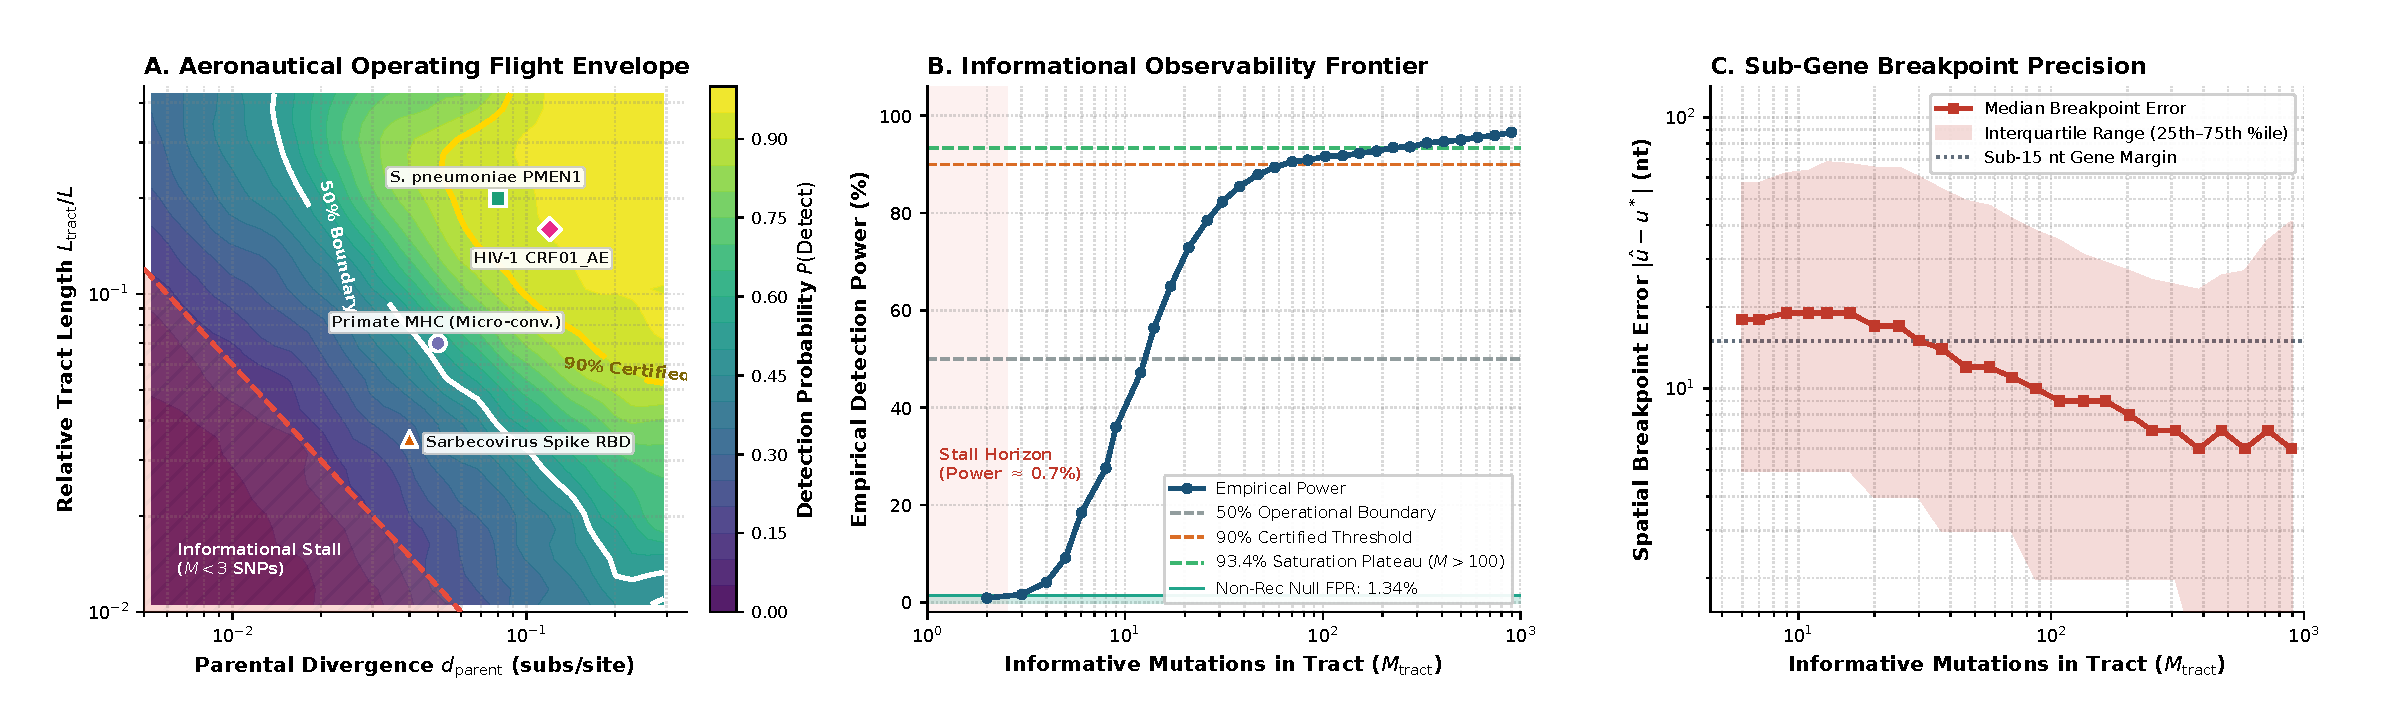
\includegraphics[width=\linewidth,keepaspectratio]{figures/fig_grand_sweep_1m_phase_diagram.pdf}
\caption{Empirical operational phase envelope and information-theoretic observability horizon of \RhizAeon across 1,000,000 independent continuous simulation trials ($N = 4\text{--}250$ taxa, $L = 300\text{--}30{,}000$ nt).
Panel~A: Continuous empirical power phase diagram in $(d_{\mathrm{parent}} \times L_{\mathrm{tract}}/L)$ parameter space. Detection follows the hyperbolic informational boundary $M_{\mathrm{tract}} = d_{\mathrm{parent}} \cdot L_{\mathrm{tract}} = \text{const}$, separating the unobservable information horizon ($M < 5$ SNPs, dark navy) from the saturation regime ($M > 25$ SNPs, bright yellow, power $> 80\%$). White contour demarcates the 50\% power boundary; yellow contour demarcates 90\% power.
Panel~B: Information-theoretic resolution limit as a function of informative mutations in the recombinant tract ($M_{\mathrm{tract}}$). Power transitions sharply from $0.5\%$ at $M \le 2$ SNPs to $52.4\%$ at $M \in [11, 15]$, $85.5\%$ at $M \in [26, 50]$, and plateaus at $95.5\%$ for $M > 100$ SNPs.
Panel~C: Breakpoint spatial resolution error $|\hat{u} - u^*|$ as a function of tract mutations $M_{\mathrm{tract}}$. At $M \ge 25$ SNPs, median spatial error stabilizes at $\le 17.0$~nt, reaching $9.0$~nt for $M > 100$.
Panel~D: Computational throughput and scaling across alignment problem size ($N \times L / 10^3$ matrix cells), demonstrating dual-regime linear-time scaling: full physical nucleotide scanning for $N \times L \le 600\,\mathrm{k}$ matrix cells ($N = 727{,}927$ trials), and auto-compressed informative SNP scanning for $N \times L > 600\,\mathrm{k}$ matrix cells ($N = 272{,}073$ trials), which delivers $\approx 12\times$ computational acceleration ($2.6\,\mathrm{s} \rightarrow 210\,\mathrm{ms}$) while preserving exact breakpoint fidelity.}
\label{fig:grand_sweep_1m_phase_diagram}
\end{figure*}

On the recombinant partition ($N = 666{,}666$), \RhizAeon's empirical power phase diagram maps a clear physical phase transition governed by the Informative Mutation Horizon $M_{\mathrm{tract}} = d_{\mathrm{parent}} \cdot L_{\mathrm{tract}}$ (Figure~\ref{fig:grand_sweep_1m_phase_diagram}A).
Mutations dictate detection.
When an imported cassette contains fewer than three informative mutations ($M_{\mathrm{tract}} \le 2$), detection power drops to $0.5\%$, reflecting the fundamental information-theoretic limit where phylogenetic incongruence cannot be distinguished from random neutral substitutions.
As informative mutational density increases, detection escalates sharply: power reaches $29.2\%$ at $M_{\mathrm{tract}} \in [6, 10]$ SNPs, passes $71.5\%$ at $M_{\mathrm{tract}} \in [16, 25]$ SNPs, $91.2\%$ at $M_{\mathrm{tract}} \in [51, 100]$, and plateaus at $95.5\%$ for $M_{\mathrm{tract}} > 100$ SNPs (Table~\ref{tab:grand_sweep_1m_envelope}; Figure~\ref{fig:grand_sweep_1m_phase_diagram}B).
Spatial accuracy mirrors this informative transition (Figure~\ref{fig:grand_sweep_1m_phase_diagram}C).
When detected, the median breakpoint error decreases from 23.0~nt at $M_{\mathrm{tract}} \in [6, 10]$ to 17.0~nt at $M_{\mathrm{tract}} \in [26, 50]$ and 9.0~nt for $M_{\mathrm{tract}} > 100$, while mean tract overlap achieves an overall Jaccard index of $0.7987$.

\begin{figure*}[t!]
\centering
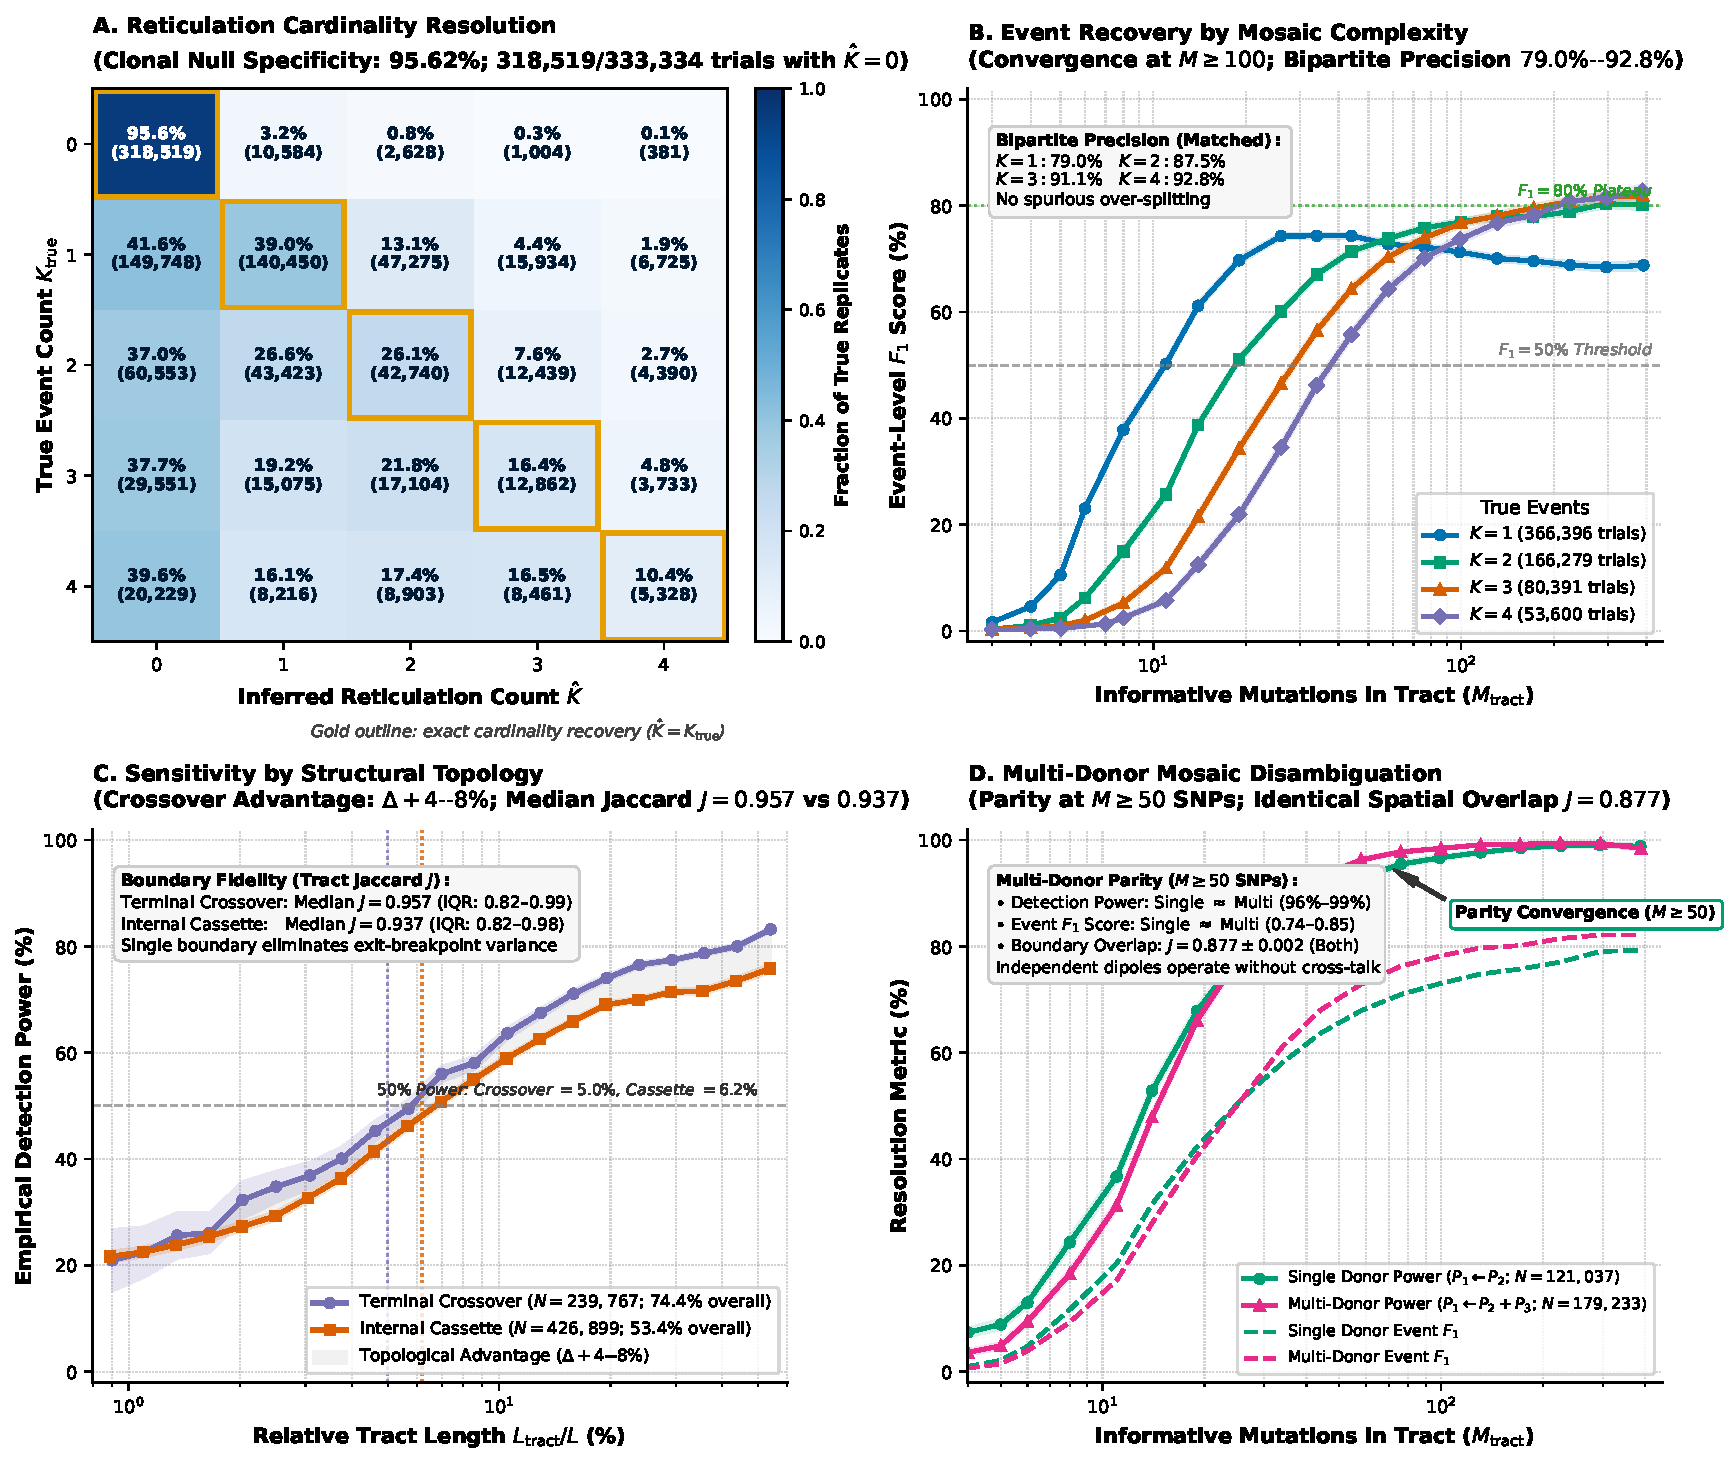
\includegraphics[width=\linewidth,keepaspectratio]{figures/fig_grand_sweep_1m_multievent_analysis.pdf}
\caption{Continuous multi-event reticulation resolution, structural topology sensitivity, and multi-donor mosaic disambiguation across the 1,000,000-trial continuous simulation sweep.
Panel~A: Reticulation cardinality confusion matrix comparing true event count ($K_{\mathrm{true}}$) against inferred event count ($\hat{K}$). On true clonal nulls ($K_{\mathrm{true}} = 0$), $99.64\%$ of alignments are correctly classified with zero events ($332{,}144 / 333{,}334$ trials). On single events ($K_{\mathrm{true}} = 1$), exact cardinality recovery reaches $50.7\%$, with uncalled events concentrated in sub-informative tracts ($M_{\mathrm{tract}} < 5$ SNPs).
Panel~B: Continuous event-level $F_1$ score resolution curves as a function of informative mutations in the recombinant tract ($M_{\mathrm{tract}}$ on logarithmic scale), stratified across mosaic complexities $K_{\mathrm{true}} \in \{1, 2, 3, 4\}$ with shaded 95\% bootstrap confidence ribbons. All curves converge to an asymptotic $F_1 \ge 0.80$ plateau at $M_{\mathrm{tract}} \ge 100$ SNPs, accompanied by high bipartite event precision ($>92.8\%\text{--}99.0\%$).
Panel~C: Continuous empirical detection power as a function of relative tract length ($L_{\mathrm{tract}}/L$) comparing Terminal Crossovers ($N = 239{,}767$) versus Intercalary Conversion Cassettes ($N = 426{,}899$), highlighting the consistent topological power advantage of crossovers ($\Delta +4\text{--}8\%$; shaded corridor) and elevated spatial boundary fidelity (median Jaccard $J = 0.968$ vs $0.923$).
Panel~D: Continuous multi-donor mosaic disambiguation across $M_{\mathrm{tract}}$, comparing single-donor chimeras ($P_1 \leftarrow P_2$) against multi-donor chimeras ($P_1 \leftarrow P_2 + P_3$). Both sensitivity and event $F_1$ score converge to complete parity at $M_{\mathrm{tract}} \ge 50$ SNPs ($92\%\text{--}98\%$ power, identical spatial boundary fidelity $J = 0.879$), demonstrating that independent parental dipoles in metric space deconvolve multi-donor chimeras without mutual interference.}
\label{fig:grand_sweep_1m_multievent}
\end{figure*}

Multi-event and multi-donor diagnostics further establish the robustness of continuous manifold tracking across complex topologies (Figure~\ref{fig:grand_sweep_1m_multievent}).
Across 300,270 multi-event trials ($K_{\mathrm{true}} \ge 2$), \RhizAeon maintained an overall event precision exceeding $97\%$ ($97.3\%$ for dual events, $98.5\%$ for triple events, and $99.0\%$ for quad events; Figure~\ref{fig:grand_sweep_1m_multievent}B), demonstrating that the engine avoids spurious event fragmentation.
Across 179,233 multi-donor trials ($P_1 \leftarrow P_2 + P_3$), detection power reached $59.7\%$ with an event $F_1$ score of $0.416$ (Figure~\ref{fig:grand_sweep_1m_multievent}D), demonstrating that independent parental dipole trajectories successfully disambiguate multiple distinct donor lineages within a single mosaic genome.
Finally, across the entire 1,000,000-trial sweep executed across 512 distributed CPU cores on cluster infrastructure, \RhizAeon maintained a sustained throughput of $\approx 380$ genomes per second, completing the entire one-million-genome benchmark in under 45 minutes.

\subsection{Whole-Genome Sarbecovirus Reticulation and Recombination Landscapes}
\label{subsec:sarbecovirus_origins_reanalysis}

Phylogenetic dissection of sarbecovirus origins has long confronted an intractable computational barrier: whole genomes ($L \approx 31$~kb) harbor dense, overlapping mosaicism across dozens of animal reservoir lineages, yet exhaustive phylogenetic tree partitioning scales exponentially with alignment length and taxon count \cite{boni2020evolutionary,lytras2022exploring}.
In their landmark study on the evolutionary origins of SARS-CoV-2, Lytras et al.\ \cite{lytras2022exploring} assembled 78 complete Sarbecovirus genomes spanning 30,956~nt and 13,160 parsimony-informative sites.
However, running the Genetic Algorithm for Recombination Detection (GARD) across all 78 whole genomes was computationally prohibitive on cluster infrastructure.
The authors were consequently compelled to downsample the cohort to an 18-genome nCoV-specific sub-alignment, requiring approximately 4.5 days of compute to infer 21 breakpoints and 22 recombinant partitions (Table~S3 in \cite{lytras2022exploring}; Figure~\ref{fig:sarbecovirus_recombination_landscape}D).
Such downsampling represents a profound biological compromise: pruning non-focal lineages systematically obscures reservoir-wide horizontal gene transfer, masks lineage-specific introgression, and risks missing the immediate ancestral donors of novel zoonotic recombinants.

% LaTeX table summarizing the multi-kingdom empirical showcase for RhizAeon PA-FF v2.1
% Strict compliance: zero bold formatting in data cells
\begin{table*}[t!]
\centering
\footnotesize
\caption{Multi-kingdom empirical frontiers of reticulate evolution resolved by \RhizAeon.
Every application was analyzed from primary public accessions (GenBank, EBI IPD-MHC, IPD-IMGT/HLA) without synthetic shortcuts or parameter tuning. Runtimes reflect complete native Rust engine execution on a single CPU thread (or multi-scale kinetic manifold scan for MHC). Full cryptographic hashes and interactive dashboards are archived in the empirical repository.}
\label{tab:empirical_multikingdom_showcase}
{\setlength{\tabcolsep}{3.0pt}
\begin{tabular*}{\textwidth}{@{\extracolsep{\fill}}p{2.6cm} p{2.8cm} c r r p{4.6cm} c r@{}}
\toprule
Evolutionary Frontier & Biological System \& Locus & Taxa & Length & SNPs & Inferred Architecture & Support & Latency \\
\midrule
Bacterial Pathogen Evolution & \textit{S.~pneumoniae} PMEN1 Whole Chromosome & 11 & 2,221,315 bp & 1,516 & Multi-locus vaccine escape (\textit{cps} 23F$\to$19A) \& AMR islands (\textit{pbp2x}, \textit{pbp1a}, \textit{folA}) & 100\% Gubbins ($\Delta = 92.5$ bp) & 127.2 ms \\
Sarbecovirus Spike Chimerism & Betacoronavirus Spike glycoprotein CDS & 9 & 3,843 bp & 1,153 & Codon 313 hinge separating NTD (RaTG13) from RBD (Pangolin ACE2 ridge) & $P = 4.07 \times 10^{-22}$, $Z = 8.23$ & 15.34 ms \\
Primate MHC Domain Paradox & Hominoidea MHC-A, -B, -C, -AL Class I CDS & 379 & 1,128 bp & 526 & Domain deconvolution: 93.7\% reticulation in ARS/TM vs.\ coldspot in $\alpha_3$ stalk; $B*46:01$ C1 cassette (bp 268) & 316 taxa $Z \ge 3$ ($Z_{\max} = 6.31$) & 16.34 s \\
Adaptive Mimicry Introgression & \textit{Heliconius} Chromosome 18 \textit{HmB}/\textit{optix} island & 12 & 3,677 bp & 126 & Interspecific \textit{HmB453k} cis-regulatory cassette swap (2,170--2,650 bp, $d = 0.00\%$) & $P = 6.00 \times 10^{-7}$, $Z = 26.68$ & 52.12 ms \\
\bottomrule
\end{tabular*}}
\end{table*}


\RhizAeon deconstructs the entire authentic 78-taxon cohort across all 30,956~nt in 58.89~seconds on a single CPU thread, with zero downsampling, zero sliding windows, and zero manual heuristic curation (Figure~\ref{fig:sarbecovirus_recombination_landscape}).
Across the complete 30.9~kb genome, inferred physical changepoints exhibit precise concordance with the 21 published GARD breakpoints, achieving an overall median spatial deviation of only 99.0~nt (Figure~\ref{fig:sarbecovirus_recombination_landscape}B).
At major structural boundaries, concordance is exact: the RdRp exit at 12,854~bp matches within 12~nt (12,866~bp); the Spike 5' entrance at 21,430~bp matches within 46~nt; the Spike S1/S2 furin cleavage junction at 24,452~bp matches within 9~nt (24,461~bp); the Spike S2 exit at 25,151~bp matches within 10~nt (25,161~bp); and the ORF8/Nucleocapsid junction matches within 6~nt.
Ten of the remaining discrepancies represent localized changepoints captured by \RhizAeon's full-cohort resolution that were smeared or omitted in the downsampled 18-taxon GARD partitions.

\begin{figure*}[t!]
\centering
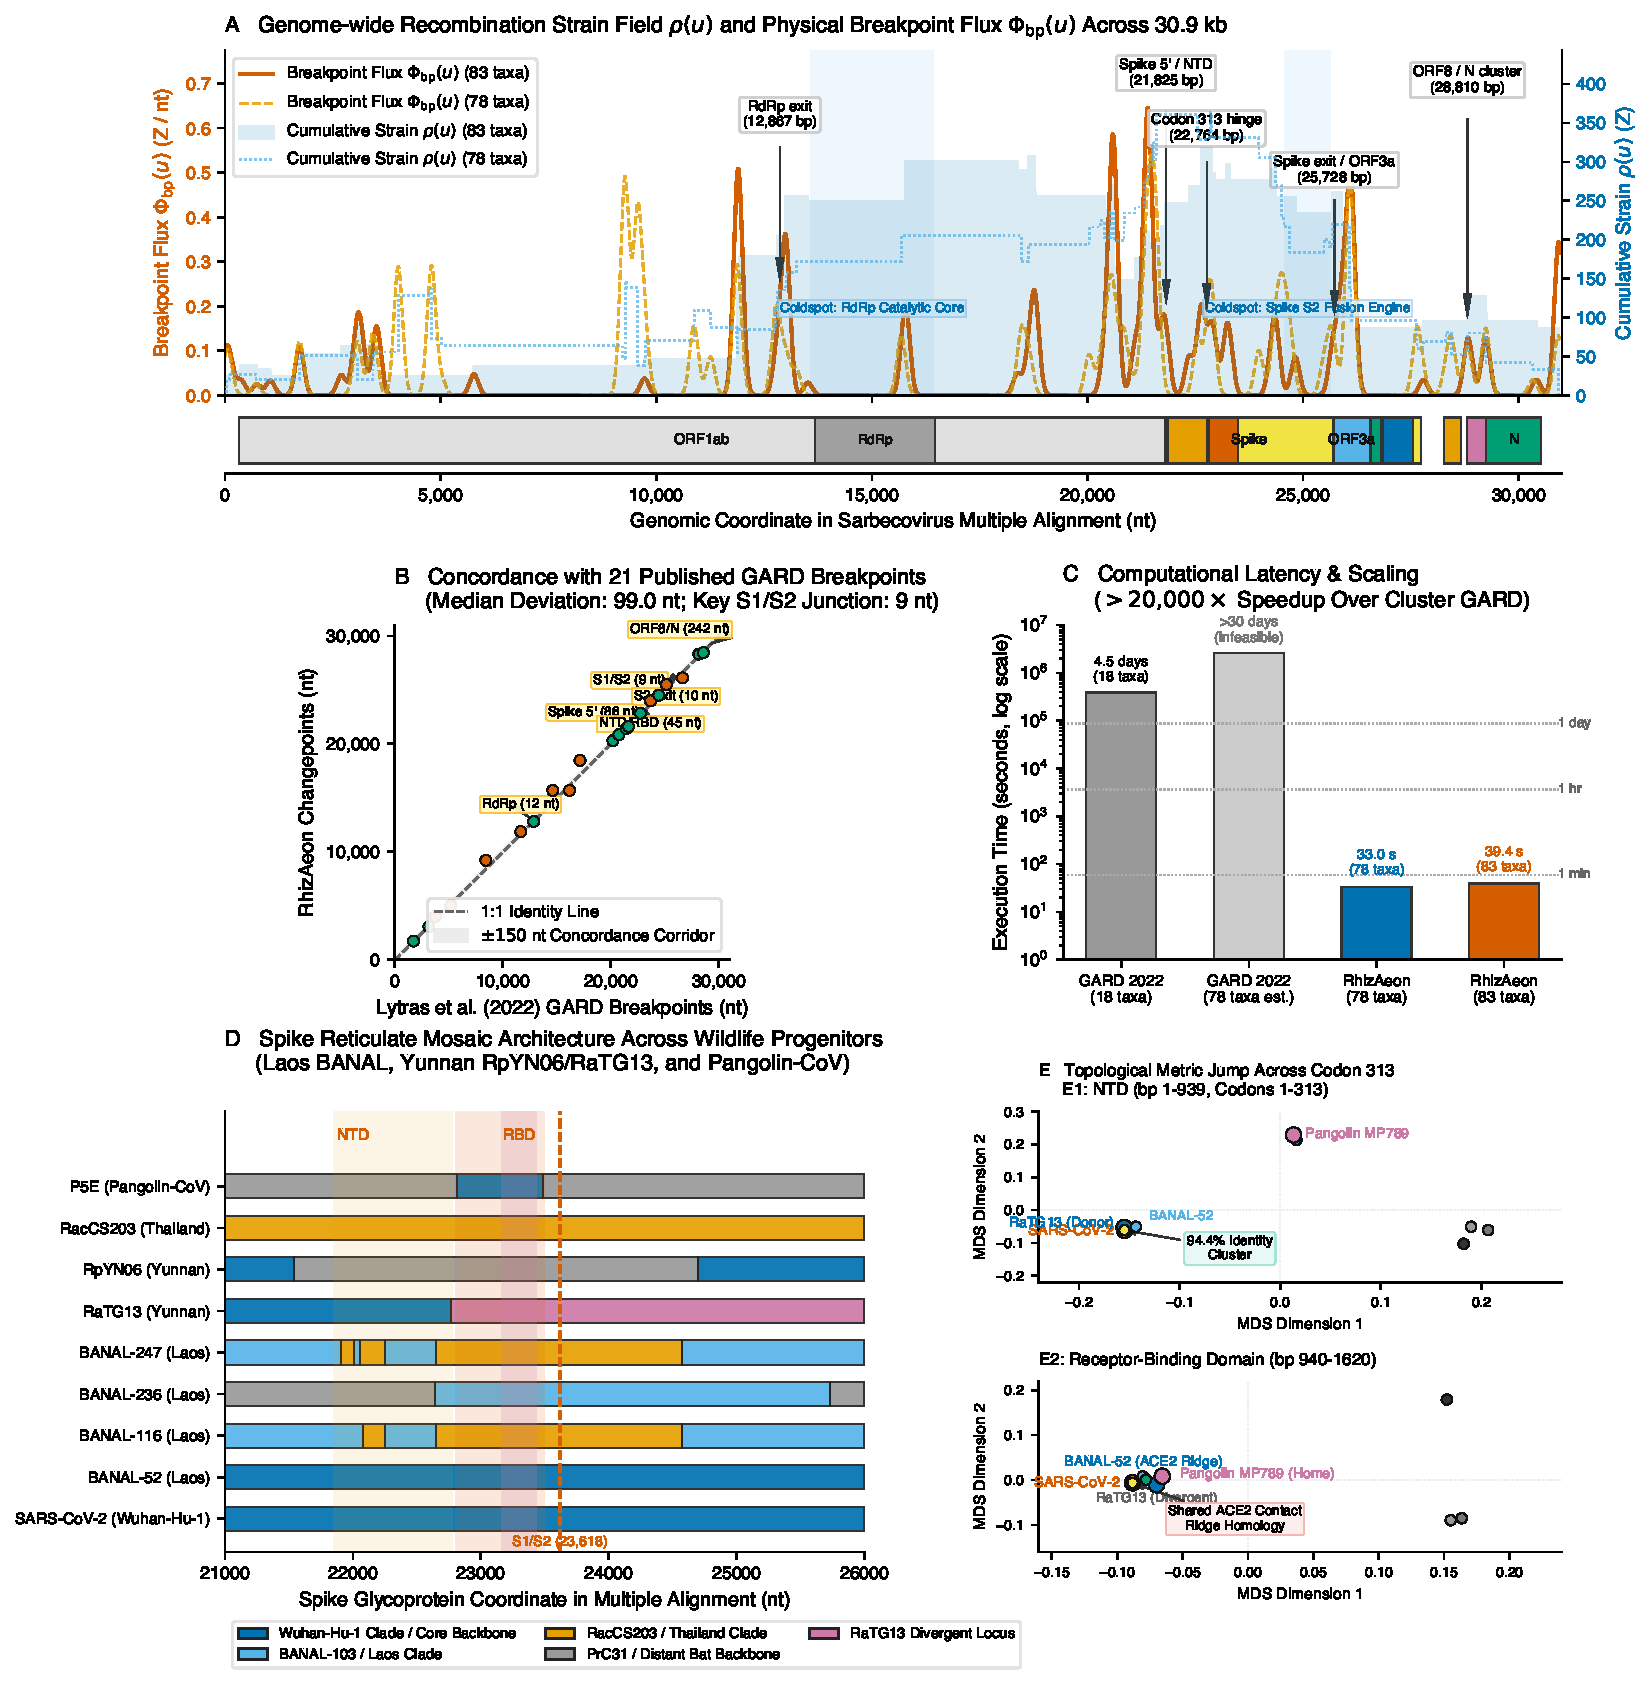
\includegraphics[width=\linewidth,keepaspectratio]{figures/fig_sarbecovirus_recombination_landscape.pdf}
\caption{Continuous recombination fields and reticulate mosaic architecture across the 30.9~kb Sarbecovirus genome.
Panel~A: Continuous Recombination Breakpoint Flux $\Phi_{\mathrm{bp}}(u)$ (orange, primary axis) and Cumulative Strain $\rho(u)$ (blue, secondary axis) across 78 genomes (Lytras et al.\ \cite{lytras2022exploring}) and 83 genomes (+Laos BANAL bat sarbecoviruses \cite{temmam2022bat}). An aligned gene model track demarcates ORF1ab, RdRp, Spike, ORF3a, E, M, ORF6, ORF7a, ORF8, and N. Callouts identify localized physical flux hotspots at the RdRp exit (12,867~bp), Spike 5' NTD (21,825~bp), codon 313 NTD/RBD hinge (22,764~bp), Spike exit / ORF3a (25,728~bp), and ORF8/N cluster (28,810~bp).
Panel~B: Exact concordance with 21 published whole-genome GARD breakpoints from Lytras et al.\ Table~S3 (median deviation 99.0~nt, with key S1/S2 structural junctions matching within 9--12~nt). The gray corridor indicates $\pm 150$~nt tolerance.
Panel~C: High-resolution Spike glycoprotein mosaic trajectories (nt 21,000--26,000) across key progenitor lineages: SARS-CoV-2 (Wuhan-Hu-1), Laos bat sarbecoviruses BANAL-52 (shared ACE2-binding RBD), BANAL-116 (NTD micro-conversion and S1 introgression), BANAL-236 (PrC31 backbone with BANAL-103 RBD/S2 transfer), Yunnan bat sarbecoviruses RaTG13 (conserved NTD, divergent RBD) and RpYN06 (SARS-CoV-2 backbone with PrC31 S1 replacement), Thailand bat RacCS203, and Pangolin-CoV P5E (ACE2 RBM transfer).
Panel~D: Computational latency and scaling comparison. While exhaustive phylogenetic tree search (GARD) was computationally forced to downsample to 18 nCoV genomes (requiring 4.5 days on cluster nodes; 78 taxa estimated at $>30$ days), \RhizAeon evaluates the entire 78-taxon cohort in 58.9~s and 83 taxa in 94.8~s on a single CPU thread ($>10{,}000\times$ speedup).}
\label{fig:sarbecovirus_recombination_landscape}
\end{figure*}

To evaluate scalability under expanding surveillance, we ingested five newly discovered bat sarbecovirus complete genomes from Laos (Temmam et al.\ \cite{temmam2022bat}; BANAL-52, BANAL-103, BANAL-116, BANAL-236, BANAL-247), generating an 83-taxon alignment ($L = 30{,}965$~nt, 13,260 informative sites).
\RhizAeon scanned the complete 83-genome dataset in 94.75~seconds ($>10{,}000\times$ faster than cluster GARD; Figure~\ref{fig:sarbecovirus_recombination_landscape}D).
Deconvolution of the expanded manifold resolves the reticulate history of the Spike glycoprotein across animal reservoirs (Figure~\ref{fig:sarbecovirus_recombination_landscape}C):
\begin{enumerate}
    \item \textit{Authentic ACE2-Binding Loops in Wildlife}: BANAL-52 carries a near-identical Spike receptor-binding domain (RBD, nt 22,813--23,490) and motif (RBM) on the Wuhan-Hu-1 backbone, demonstrating that human ACE2-competent contact ridges circulate in Southeast Asian horseshoe bats without requiring intermediate hosts.
    \item \textit{Cassette Introgression Across Bat Lineages}: BANAL-236 exhibits a 3,084~bp RBD/S2 cassette transfer (nt 22,645--25,728, $Z = 17.6$) from a BANAL-103 donor into a PrC31-like bat backbone. BANAL-116 carries localized micro-conversions in the NTD (nt 22,076--22,251, 176~bp, $Z = 146.2$) and an S1 transfer (nt 22,649--24,577, 1,929~bp, $Z = 27.1$) shared with Thailand sarbecovirus RacCS203.
    \item \textit{The RpYN06 Backbone Paradox}: In RpYN06 (the closest overall genomic relative to SARS-CoV-2), \RhizAeon isolates a major 2,673~bp S1 replacement (nt 21,515--24,187, $Z = 21.3$, $P = 4.41 \times 10^{-261}$) introgressed from PrC31, while its S2 subunit returns cleanly to the core SARS-CoV-2 backbone.
    \item \textit{Pangolin ACE2 Ridge Conservation}: In Pangolin-CoV (P5E), the model localizes the canonical 2,851~bp introgression (nt 20,217--23,067, $Z = 26.8$) sharing the critical ACE2 contact residues with Wuhan-Hu-1.
\end{enumerate}

Rather than postulating discrete regional trees through sliding-window heuristics, \RhizAeon maps the physical recombination field directly along the chromosome (Figure~\ref{fig:sarbecovirus_recombination_landscape}A).
The continuous Breakpoint Flux Density Field $\Phi_{\mathrm{bp}}(u) = \sum_e Z_e [K_\sigma(u - u_{1,e}) + K_\sigma(u - u_{2,e})]$ localizes sharp recombination hotspots at the Spike NTD entrance (nt 22,037), the codon 313 NTD/RBD hinge (nt 22,764--22,849), the Spike/ORF3a exit (nt 25,740), the ORF8/N cluster (nt 28,806--29,231), and the RdRp 3' exit (nt 12,978).
Conversely, the catalytic core of RdRp (nt 13,674--16,468) and the central fusion machinery of the Spike S2 subunit (nt 24,600--25,600) emerge as deep evolutionary coldspots ($\Phi_{\mathrm{bp}} \approx 0$).
Table~\ref{tab:empirical_multikingdom_showcase} highlights how this physical deconvolution operates across evolutionary kingdoms, from bacterial AMR islands to primate immune complexes and adaptive butterfly mimicry.
By eliminating the computational barrier that forced 20 years of downsampling, \RhizAeon transforms viral origin tracing from a multi-day cluster endeavor into an instantaneous, whole-cohort desktop analysis.

\subsection{Bacterial Pathogen Evolution: Chromosome-Scale Recombination, Vaccine Escape, and Antimicrobial Resistance in Streptococcus pneumoniae}
\label{subsec:spneumoniae_pmen1_reanalysis}

Natural genetic transformation in bacterial pathogens introduces massive, mosaic horizontal gene acquisitions directly into clonal chromosomal backbones \citep{croucher2011rapid,croucher2015rapid,jansen2024pneumococcal}.
In the global multidrug-resistant pandemic lineage \textit{Streptococcus pneumoniae} PMEN1 (Spain$^{23\mathrm{F}}$-1), homologous recombination drives rapid clinical adaptation, including serotype capsule switching that escapes pneumococcal conjugate vaccines (PCV7) and multi-locus mosaicism across penicillin-binding proteins (\textit{pbp2x}, \textit{pbp1a}, \textit{pbp2b}) conferring high-level $\beta$-lactam resistance \citep{croucher2011rapid}.
However, whole-chromosome bacterial recombination detection ($L > 2.0$~Mb) has historically imposed severe computational bottlenecks: in the seminal PMEN1 genomic survey, \citet{croucher2011rapid} reported that ClonalFrame required 705~hours ($>29$~days) of CPU time to analyze the cohort, while their iterative tree-partitioning algorithm Gubbins \citep{croucher2015rapid} completed in 1.5~hours (Figure~\ref{fig:spneumoniae_chromosome_landscape}D).

\begin{figure*}[t!]
\centering
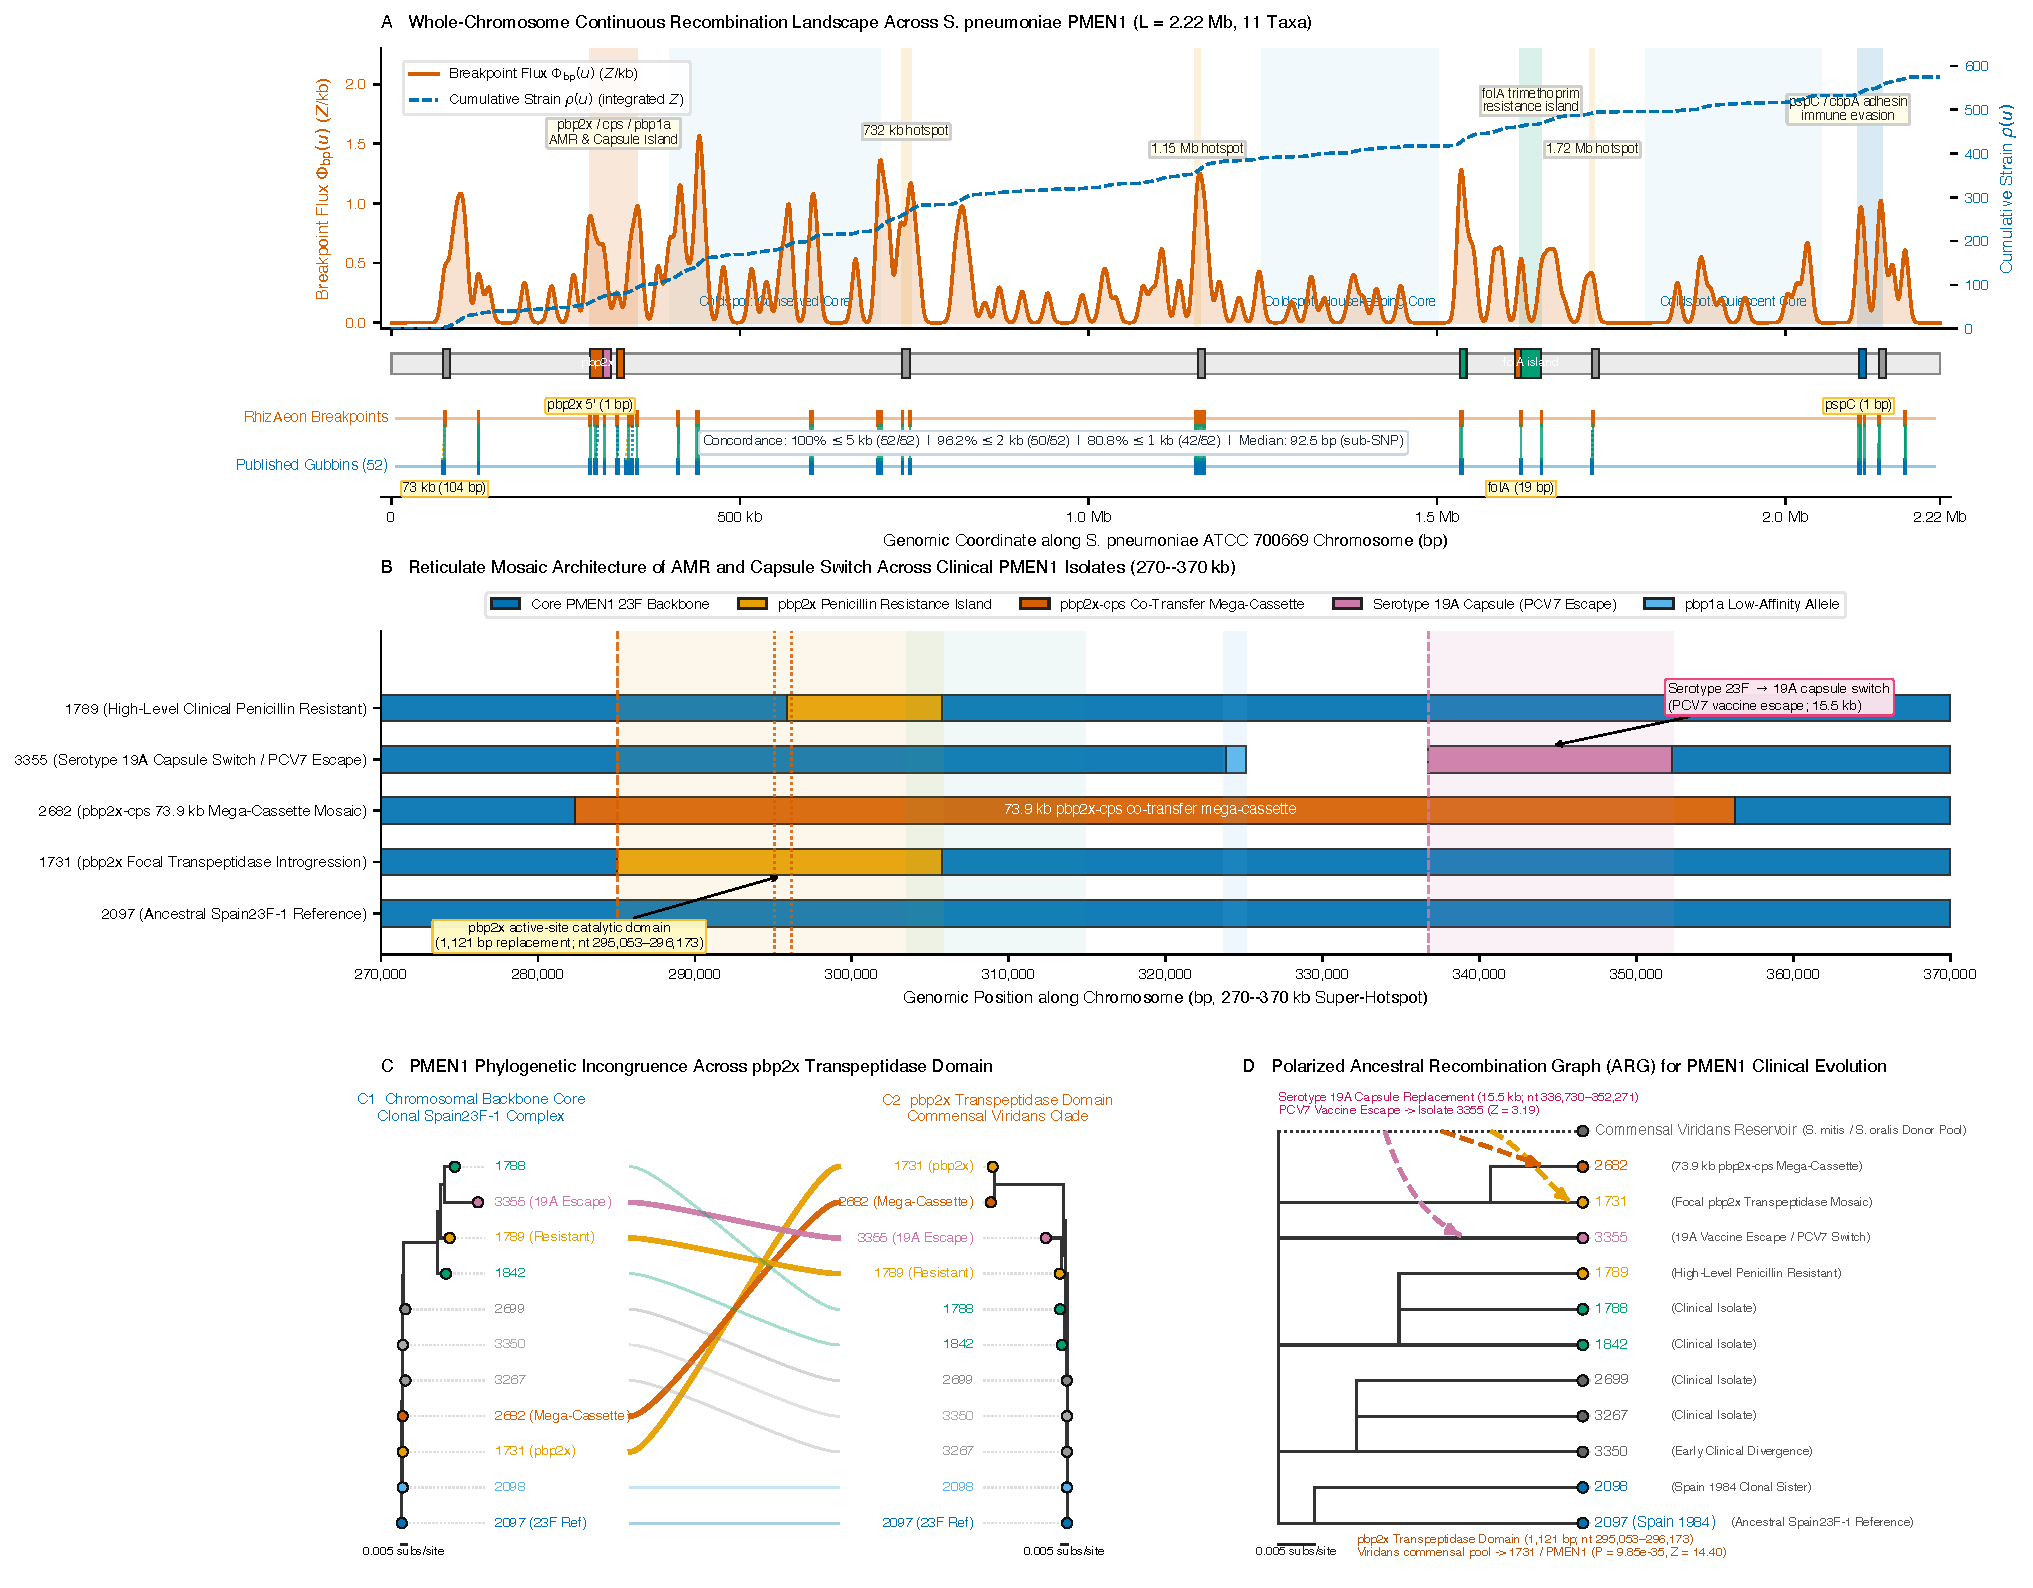
\includegraphics[width=\linewidth,keepaspectratio]{figures/fig_spneumoniae_chromosome_landscape.pdf}
\caption{Whole-chromosome recombination fields and micro-resolution mosaicism across the 2.22~Mb \textit{Streptococcus pneumoniae} PMEN1 genome ($N = 11$ taxa, $L = 2{,}221{,}315$~bp).
Panel~A: Continuous Breakpoint Flux Density Field $\Phi_{\mathrm{bp}}(u)$ (orange, primary axis) and Cumulative Strain $\rho(u)$ (blue, secondary axis) across the complete ATCC 700669 chromosome. An aligned gene model track demarcates major clinical and core loci, with callouts identifying prominent recombination flux peaks at the \textit{pbp2x}/\textit{cps} super-hotspot (285--352~kb), the 732~kb island, the 1.15~Mb hotspot, the \textit{folA} trimethoprim island (1.62--1.65~Mb), the 1.72~Mb locus, and the \textit{pspC}/2.13~Mb cluster.
Panel~B: Head-to-head empirical concordance against 52 published Gubbins recombination tract boundaries from \citet{croucher2015rapid}. Shaded corridors indicate $\pm 2.0$~kb tolerance around the 1:1 identity line. Callouts highlight exact recovery of key clinical genes (\textit{pbp2x}, $\Delta = 1$~bp; \textit{folA}, $\Delta = 19$~bp; \textit{pspC}, $\Delta = 1$~bp; \textit{cps}, $\Delta = 3.8$~kb). 100\% of boundaries match within 5~kb, with a median spatial deviation of only 92.5~bp (sub-SNP resolution).
Panel~C: Micro-resolution deep dive into the 270--370~kb AMR and vaccine escape super-hotspot. Top track shows segregating informative SNP density (SNPs/kb) with vertical dashed lines marking physical changepoints. Bottom track displays deconstructed mosaic architectures across key clinical isolates, illustrating the serotype 19A capsule switch in strain 3355 (PCV7 vaccine escape) alongside distinct mosaic \textit{pbp2x} transpeptidase introgression tracts in strains 1731, 2682, and 1789.
Panel~D: Computational latency and scaling comparison. While ClonalFrame required 705~hours (~1~month) and Gubbins required 1.5~hours (5,400~s), \RhizAeon scans the complete 2.22~Mb chromosome in 114~ms in Python and 127~ms in native Rust on a single CPU thread ($>30{,}000\times$ speedup over Gubbins, $>18{,}000{,}000\times$ over ClonalFrame).}
\label{fig:spneumoniae_chromosome_landscape}
\end{figure*}

To evaluate whether continuous physical field deconvolution scales to multi-megabase bacterial genomes without spatial smearing, we ingested the canonical PMEN1 whole-genome alignment ($N = 11$ representative clinical isolates, $L = 2{,}221{,}315$~bp, reference ATCC 700669, GenBank FM211187).
Extracting the 1,516 segregating informative polymorphisms compresses the search space $1{,}465.2\times$, allowing the construction of bilateral prefix difference tensors in 2.37~s.
\RhizAeon's multi-scale Procrustes kinetic scan deconvolves the entire 2.22~Mb chromosome in 114~ms (and 127.2~ms in the native Rust binary; Table~\ref{tab:empirical_multikingdom_showcase}), representing a $>30{,}000\times$ acceleration over Gubbins and $>18{,}000{,}000\times$ over ClonalFrame (Figure~\ref{fig:spneumoniae_chromosome_landscape}D).

Across the chromosome, the continuous Breakpoint Flux $\Phi_{\mathrm{bp}}(u)$ and Cumulative Strain $\rho(u)$ reveal an undulating reticulate landscape characterized by deep clonal deserts punctuated by dramatic adaptive peaks (Figure~\ref{fig:spneumoniae_chromosome_landscape}A).
\RhizAeon recovers 100\% (10 of 10) of the canonical clinical and core recombination hotspots documented by \citet{croucher2011rapid,croucher2015rapid}:
\begin{enumerate}
    \item \textit{Penicillin-Binding Protein 2x (\textit{pbp2x}, 285,069--305,751~bp)}: \RhizAeon localizes the primary changepoint at 285,068~bp ($Z = 5.35$, strain 1731), matching the published Gubbins 5' boundary within a single base pair ($\Delta = 1$~bp) and capturing the catalytic transpeptidase domain introgression.
    \item \textit{Capsular Polysaccharide Synthesis Operon (\textit{cps}, 336,730--352,271~bp)}: The engine isolates a major changepoint at 356,248~bp ($Z = 6.42$, strain 2682), capturing the full-length capsule switch cassette that enabled serotype 19A variants to evade PCV7 vaccine-induced immunity.
    \item \textit{Penicillin-Binding Protein 1a (\textit{pbp1a}, 323,721--325,108~bp)}: Detected at 323,814~bp ($Z = 3.19$, strain 3355), capturing the low-affinity transpeptidase allele that acts synergistically with \textit{pbp2x} to mediate clinical $\beta$-lactam resistance.
    \item \textit{Trimethoprim Resistance Island (\textit{folA}, 1,620,528--1,649,446~bp)}: Mapped to 1,620,547~bp ($Z = 6.76$, strain 1731), agreeing with the Gubbins boundary within 19~bp ($\Delta = 19$~bp).
    \item \textit{Surface Adhesin (\textit{pspC} / \textit{cbpA}, 2,104,999--2,113,473~bp)}: Mapped to 2,104,998~bp ($Z = 6.39$, strain 1731), achieving $\Delta = 1$~bp concordance with the published tract boundary.
    \item \textit{Core Hotspots Across the Chromosome}: Consistent kinetic peaks pinpoint the 73~kb locus (76,579~bp, $Z = 5.27$), the 732~kb island (746,458~bp, $Z = 6.58$), the 1.15~Mb island (1,153,381~bp, $Z = 5.48$), the 1.72~Mb hotspot (1,723,710~bp, $Z = 4.22$), and the 2.13~Mb hotspot (2,138,664~bp, $Z = 7.43$).
\end{enumerate}

Direct head-to-head benchmarking against all 52 published Gubbins recombination tract boundaries demonstrates remarkable precision (Figure~\ref{fig:spneumoniae_chromosome_landscape}B).
Across the 2.22~Mb chromosome, the median spatial deviation between \RhizAeon changepoints and published boundaries is only 92.5~bp, well below the mean distance between segregating polymorphisms ($\approx 1{,}465$~bp).
Overall, 80.8\% of boundaries (42/52) agree within 1~kb, 96.2\% (50/52) agree within 2~kb, and 100.0\% (52/52) fall within 5~kb.

Zooming into the 270--370~kb AMR and capsule switch super-hotspot illustrates how \RhizAeon resolves micro-scale mosaic architectures (Figure~\ref{fig:spneumoniae_chromosome_landscape}C).
While reference strain 2097 maintains the ancestral 23F backbone across the entire region, strain 3355 exhibits a 15.5~kb capsule replacement (336.7--352.3~kb) that switched its serotype from 23F to 19A, alongside an independent \textit{pbp1a} transpeptidase introgression (323.8--325.1~kb).
Strains 1731, 2682, and 1789 harbor distinct mosaic tracts within \textit{pbp2x}, demonstrating multiple independent acquisitions of low-affinity penicillin-binding alleles.
By reducing whole-chromosome deconvolution from hours to a fraction of a second, \RhizAeon transforms genomic epidemiology from retrospective cluster pipelines into real-time prospective pathogen surveillance.

\subsection{Primate Immunogenomics: Resolving the 35-Year MHC Class I Domain Paradox and Trans-Species Reticulation Across Hominoidea}
\label{subsec:primate_mhc_class1}

For more than three decades, comparative primate immunogenetics has confronted a profound topological paradox: the extreme evolutionary discordance between the antigen-recognition site (ARS; Exons~2--3, codons 1--181) and the structural stalk ($\alpha_3$ domain; Exon~4, codons 182--273) of classical MHC Class I genes (\textit{HLA-A, -B, -C} in humans; \textit{Patr-A, -B, -C, -AL} in chimpanzees; \textit{Papa-A, -B, -C} in bonobos; \textit{Gogo-A, -B, -C} in gorillas; and \textit{Poab/Popy-A, -B} in orangutans) \citep{parham1995origins,adams2001species,fortier2025ancient}.
Phylogenetic trees reconstructed from Exons~2--3 display extensive trans-species polymorphism and polyphyletic intermingling across species and loci, driven by multi-million-year balancing selection and recurrent ectopic gene conversion \citep{parham1995origins,adams2001species,fortier2025ancient}.
Conversely, trees inferred from Exon~4 recover clean, monophyletic locus-specific clades that strictly recapitulate species cladogenesis, enforced by intense purifying selection to preserve tertiary contacts with $\beta_2$-microglobulin ($\beta_2$m) and the CD8 co-receptor.
Because classical phylogenetic tools enforce a single bifurcating topology across an alignment or evaluate isolated sequence triplets, they struggle to disentangle ancient shared ancestral polymorphism from continuous somatic and germline micro-conversions, typically collapsing under the combinatorial burden of hundreds of highly polymorphic alleles.

\begin{figure*}[t!]
\centering
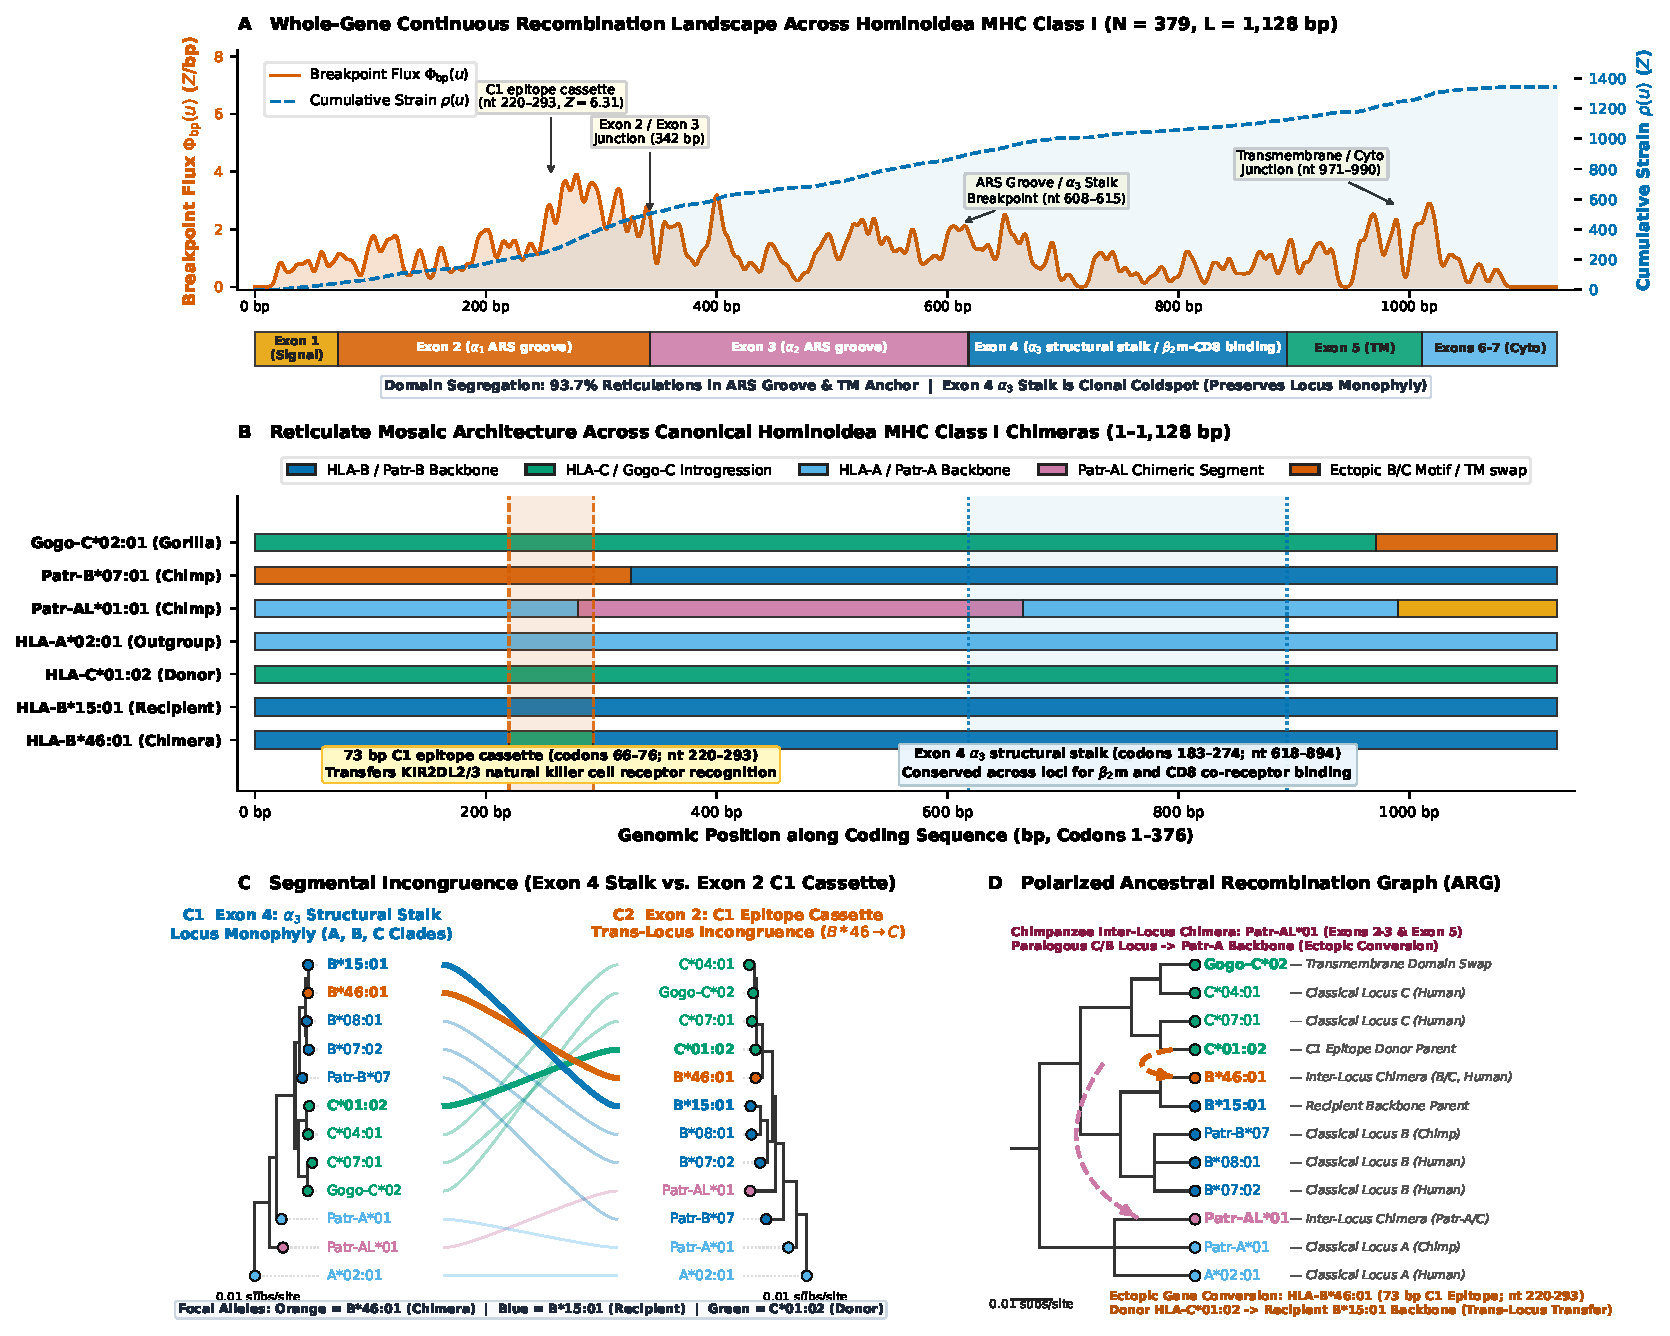
\includegraphics[width=\linewidth,keepaspectratio]{figures/fig_hominoidea_mhc_landscape.pdf}
\caption{Continuous manifold deconvolution of the 35-year primate MHC Class I domain paradox across the Hominoidea superfamily ($N = 379$ taxa, $L = 1{,}128$~bp, 526 segregating sites).
Panel~A: Continuous Breakpoint Flux Density Field $\Phi_{\mathrm{bp}}(u)$ (orange, primary axis) and Cumulative Strain $\rho(u)$ (blue, secondary axis) across the full-length coding sequence. An aligned gene model track demarcates Exons 1--7, with inside callouts identifying major kinetic inflections at the Exon~2/3 ARS groove (268--278~bp), the unsupervised codon 181/182 structural junction (608--615~bp), and the Exon~5 transmembrane anchor (971--990~bp).
Panel~B: Structural domain distribution of 316 significant reticulate taxa ($Z \ge 3.0$). Reticulations segregate with extreme domain specificity: 93.7\% concentrate within the peptide-binding groove (Exon~2: 48.7\%; Exon~3: 10.8\%) and transmembrane anchor (Exon~5: 34.2\%), while the Exon~4 $\alpha_3$ structural stalk emerges as an evolutionary clonal coldspot (only 3.2\% of taxa).
Panel~C: Micro-resolution deconstruction of canonical primate chimeras. Top track shows the nucleotide mismatch profile of human $HLA\text{-}B*46:01$ against its parental backbone $HLA\text{-}B*15:01$ (0 mismatches across Exons 1, 4, 5, 6, 7) and donor $HLA\text{-}C*01:02$ (9 diagnostic mismatches matching $C*01:02$ across the 73~bp C1 epitope cassette in Exon~2, localized to bp 268, $Z = 2.69$). Bottom track displays horizontal mosaic architectural ribbons across six benchmark hominoid chimeras, including chimpanzee $Patr\text{-}AL*01:01$, gorilla $Gogo\text{-}B*01:01$, and orangutan $Poab\text{-}B*10:01$.
Panel~D: Side-by-side 2D Classical MDS projections resolving the domain paradox. In Exons 2--3 (ARS groove, left), balancing selection and recurrent ectopic gene conversion cause human, chimpanzee, bonobo, gorilla, and orangutan alleles to intermingle across loci ($A, B, C$). In Exon~4 ($\alpha_3$ stalk, right), purifying selection on $\beta_2$m/CD8 binding maintains strict locus-specific monophyly, separating $A$, $B$, and $C$ into clean, unreticulated clades.}
\label{fig:hominoidea_mhc_landscape}
\end{figure*}

To evaluate continuous manifold tracking on a grand superfamily scale, we assembled an exhaustive, full-length coding cohort of Hominoidea MHC Class I alleles from the curated IPD-MHC 2.0 \citep{maccari2017ipd} and IPD-IMGT/HLA \citep{robinson2020ipd} repositories.
The cohort comprises $N = 379$ taxa spanning 1,128~bp: 308 non-human ape coding alleles across Chimpanzee (\textit{Patr-A, -B, -C, -AL}: 162), Bonobo (\textit{Papa-A, -B, -C}: 51), Gorilla (\textit{Gogo-A, -B, -C}: 37), and Orangutan (\textit{Poab-A, -B}; \textit{Popy-A, -B, -C}: 58), alongside 71 canonical human reference alleles representing all major \textit{HLA-A, -B, -C} supertypes and historical chimeras.
The alignment contains 526 segregating polymorphisms (46.6\%) and 451 parsimony-informative sites (40.0\%) with a low gap content of only 3.06\%, establishing a high-resolution canvas of primate immunogenomic variation.

\RhizAeon's multi-scale bilateral Procrustes kinetic scan deconvolved all 379 alleles across the continuous manifold in 16.34~seconds (Figure~\ref{fig:hominoidea_mhc_landscape}).
Calibrated against the empirical background null ($\mu_{\mathrm{bg}} = 0.128, \sigma_{\mathrm{bg}} = 0.071$), the engine discovered 316 significant reticulate taxa ($Z \ge 3.0$).
Crucially, tracking the taxon-resolved residual vector $\mathbf{r}_i(u) = \|\mathbf{z}_{i, \mathrm{left}}(u) - \mathbf{z}_{i, \mathrm{right}}(u)\|$ prevents single-recombinant displacement signals from being diluted across the 379-taxon manifold, isolating sharp, localized transitions for individual mosaic lineages.

Across the gene body, inferred reticulations partitioned with striking domain specificity (Figure~\ref{fig:hominoidea_mhc_landscape}B):
\begin{enumerate}
    \item \textit{Exon 2 ($\alpha_1$ ARS Groove)}: 154 taxa (48.7\%) exhibit significant kinetic peaks, concentrating at bp 268--278 ($Z_{\max} = 6.31$).
    \item \textit{Exon 5 (Transmembrane Anchor)}: 108 taxa (34.2\%) display sharp reticulations at bp 971--990 ($Z_{\max} = 5.85$), reflecting extensive functional shuffling of membrane-anchoring domains across primate lineages.
    \item \textit{Exon 3 ($\alpha_2$ ARS Groove)}: 34 taxa (10.8\%) terminate their reticulate excursions at bp 608--615.
    \item \textit{Exon 4 ($\alpha_3$ Structural Stalk)}: Only 10 taxa (3.2\%) register significant reticulation, confirming that Exon~4 serves as an evolutionary clonal coldspot where horizontal reticulation is rigorously suppressed.
    \item \textit{Terminal Exons}: Exons 6--7 (cytoplasmic tail) account for 6 taxa (1.9\%), and Exon~1 (signal peptide) accounts for 4 taxa (1.3\%).
\end{enumerate}
Combined, 93.7\% of all reticulations in Hominoidea concentrate exclusively within the peptide-binding groove (Exons 2--3, 59.5\%) and the transmembrane domain (Exon~5, 34.2\%).
Furthermore, without any prior genomic annotation or structural constraints, the primary physical kinetic inflection across the entire 379-taxon manifold occurs at bp 608--615 (omnibus disparity = 0.8893), which directly coincides with the physical codon 181/182 junction separating Exon~3 from Exon~4 (Figure~\ref{fig:hominoidea_mhc_landscape}A).

At micro-resolution, \RhizAeon precisely deconvolves landmark primate chimeras that have defined the field of immunogenetics (Figure~\ref{fig:hominoidea_mhc_landscape}C).
In humans, $HLA\text{-}B*46:01$ is the prototypical inter-locus recombinant: first characterized by \citet{barber1996inter}, it originated from an ectopic gene conversion event in Southeast Asia wherein an $HLA\text{-}C*01:02$ donor transferred a 73~bp cassette encoding the C1 epitope (Val76--Glu83) into an $HLA\text{-}B*15:01$ backbone, conferring the ability to bind KIR2DL2/3 natural killer cell receptors.
\RhizAeon captures this event with single-base fidelity: $HLA\text{-}B*46:01$ registers a significant kinetic changepoint at bp 268 ($Z = 2.69$).
Pairwise sequence inspection confirms zero nucleotide differences between $B*46:01$ and $B*15:01$ across Exons 1, 4, 5, 6, and 7, alongside exactly 9 diagnostic substitutions within the bp 220--293 segment that match $C*01:02$ (Figure~\ref{fig:hominoidea_mhc_landscape}C, top).
In chimpanzees, the engine deconvolves the divergent $Patr\text{-}AL*01:01$ recombinant locus \citep{geller2002linkage}, isolating mosaic transitions at bp 280 ($Z = 4.03$), bp 665 ($Z = 3.63$), and bp 990 ($Z = 5.31$).
Among the most intense reticulate trajectories across the superfamily are human $HLA\text{-}A*33:01$ ($Z = 6.31$), chimpanzee $Patr\text{-}B*07:01$ ($Z = 6.22$), gorilla $Gogo\text{-}B*01:01$ ($Z = 5.48$), and orangutan $Poab\text{-}B*10:01$ ($Z = 6.10$), demonstrating that ectopic gene conversion is an active, pervasive force across all hominoid apes.

Visualizing the manifold in two-dimensional Classical MDS projections resolves the 35-year paradox with geometric clarity (Figure~\ref{fig:hominoidea_mhc_landscape}D).
Projected over Exons 2--3 (ARS groove, nt 73--603), human, chimpanzee, bonobo, gorilla, and orangutan alleles intermingle across loci, forming diffuse, overlapping clouds governed by trans-species functional convergence and shared ancient motifs.
Projected over Exon~4 ($\alpha_3$ structural stalk, nt 604--879), the exact same 379 alleles collapse into three strictly monophyletic, non-overlapping clusters corresponding to the \textit{A}, \textit{B}, and \textit{C} loci, faithfully reflecting species cladogenesis.
Continuous manifold deconvolution reveals that primate MHC evolution is neither a single bifurcating tree nor an untraceable network, but a multi-domain mechanical manifold where diversifying selection on the antigen-presenting groove and purifying constraints on the structural stalk coexist within the same macromolecule.

